% !TEX TS-program = xelatex
% !TEX encoding = UTF-8 Unicode

\documentclass[a4paper,itemph,amsmath,oneside,11pt,openany]{xoblivoir}

\usepackage{subfig}
\usepackage{amsmath}
\usepackage{graphicx}
\usepackage{makeidx}
\usepackage{amsfonts}
\usepackage{amssymb}
\usepackage{marginnote}
\usepackage{float}

\usepackage{fapapersize}
\usefapapersize{210mm,290mm,30mm,*,35mm,30mm}

%% Font Settings
%\setmainfont[Mapping=tex-text]{TeX Gyre Termes}
%\setsansfont[Mapping=tex-text]{TeX Gyre Heros}
%\setkormainfont(* ExtraBold)(나눔고딕){나눔명조}(){바탕}
%\setkorsansfont(* Bold)(*){나눔고딕}
\setkormainfont(-윤고딕330)(*){-윤명조310}

\pagestyle{hangul}

% \setcounter{tocdepth}{3}
% \setcounter{secnumpdepth}{3}


\SetHangulspace{1.6}{1.2}
% \renewcommand{\baselinestretch}{1.6}
% \numberwithin{equation}{section}

\begin{document}

\title{지연 셰이딩 기법을 사용하는 소프트웨어 렌더러 구현과 시스템 성능 측정}
\author{류형욱(2013011037, 컴퓨터공학부 소프트웨어전공)}
\date{}
\maketitle
\tableofcontents
\section{서론}
  컴퓨터 그래픽스의 근간을 이루는 렌더링 기술은 높은 수준의 컴퓨터 공학, 수학, 물리학으로 이루어져 있으며,
많은 컴퓨팅 파워가 필요하여 하드웨어와 소프트웨어 성능을 빠르게 발전시키는 역할을 하고 있다.

렌더링에는 레이 트레이싱, 포톤 매핑, 폴리곤 기반 래스터라이제이션과 같은 방법이 주로 사용된다.
오늘날 크게 높아진 하드웨어 성능으로 인해 과거에는 실현하기 어려웠던 렌더링 방법이 실시간 렌더링 방법으로 사용되기도 하고,
광선 추적법과 같이 과거 CPU만이 수행할 수 있었던 렌더링 방법을 GPU에서 실행할 수 있도록 하는 하드웨어 지원도 등장하였다.

특히 폴리곤 기반 래스터라이제이션은 실시간 렌더링에서 가장 널리 쓰이는 방법이며, 연산의 복잡도가 낮고 병렬화가 간단해
주로 하드웨어에서 실행되고, 하드웨어 가속기가 일반화된 이후 소프트웨어 구현은 거의 사용하지 않는다.
하지만, 고정 파이프라인을 제거하고 프로그래밍 가능한 셰이더 모델이 도입된 최근에도 하드웨어를 사용하는 렌더링은
소프트웨어 렌더링에 비하여 구현의 자유도 측면에서 제약 사항이 많다. 모든 연산이 CPU에서 실행되는 소프트웨어 렌더러가
하드웨어 가속기의 렌더링 파이프라인과 유사한 실행 구조를 가지면서 느리게 동작한다고 할지라도, 미리 제공되는 API 뒤에
감추어져 있던 컴퓨터 그래픽스의 재미를 찾고 자유롭게 파이프라인을 설계해 보는 것은, 여전히 가치가 있는 일이다.

한편, 최근 출시되는 게임에서는 다양한 동적 광원을 적은 부하로 사용하기 위하여 지연 셰이딩을 사용하는 사례가 많다.
반면에 상용 게임 개발이 현실적으로 불가능한 소프트웨어 렌더링에 대해서는 지연 셰이딩이나 지연 라이팅과 같은
기술이 적용된 사례를 찾아볼 수 없었다.

본 소논문에서는 순수하게 CPU에서 동작하고 지연 셰이딩 기법을 사용하는 소프트웨어 렌더러를 구현해 보고,
개발 속도와 용이성 관점에서 하드웨어를 사용하는 구현과 비교해 본다. 또, 소프트웨어 렌더링의 특징을 활용한
시스템 성능 측정 소프트웨어로의 활용 가능성에 대해 알아본다.

\section{시험 모델}
  연구에서 렌더링을 시험할 대표 모델로, TF3DM\footnote{\cite{model}Balmung, Iron Man Mark 7, http://tf3dm.com/3d-model/iron-man-mark-7-81052.html}에서
공개 배포되고 있는 ``아이언 맨 마크 7''을 3D 모델로 사용하였다. 이 3D 모델은 굴곡과 매끄러운 면을 적당히 가지고 있다.
또, 느린 소프트웨어 렌더러에서 짧은 시간 안에 렌더링하기에 폴리곤 수가 적당하다.

\begin{figure}[H]
\centering
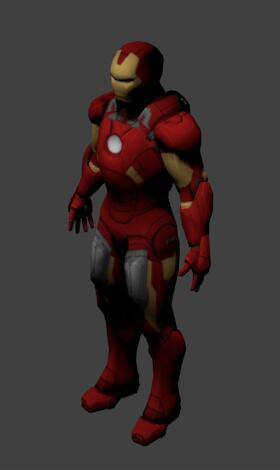
\includegraphics[width=40mm]{img/model}
\caption{Blender에서 렌더링한 시험 모델}
\end{figure}


\section{렌더링 기하}
  렌더링은 선형대수학에 바탕을 두고 있으며, 최종 이미지를 그리기 위해서 많은 양의 벡터와 행렬,
행렬과 행렬 사이의 연산이 수행된다. 렌더링에는 2차원, 3차원, 4차원 벡터가 사용되며, 여러 가지 이유로
실제 연산에서는 마지막 성분을 1로 설정한 4차원 벡터를 사용하며, 행렬에서도 마찬가지로 4행 4열 행렬을 주로 사용한다.
벡터와 행렬 연산의 성질과 선형성에 따라 복잡한 작업을 일관되고 빠르게 수행할 수 있다. 예를 들어, 여러 단계로 이루어진
선형 변환을 합성하고 한 번에 처리하여 프로그램의 복잡도와 수행 시간에서 이득을 얻는다.\footnote{\cite{korea}James D. Foley, Andries van Dam, Steven K. Feiner, John F. Hughes, Richard L. Phillips, 조동섭, 한정현 옮김, 컴퓨터 그래픽스, 홍릉과학출판사, 1998, p.178}

폴리곤, 특히 삼각형에 속한 정점들은 변환 행렬과의 연산을 통해 다른 점으로 이동되고, 최종적으로는 화면상의 공간으로 옮겨지며,
래스터라이저가 삼각형을 래스터라이징함에 따라서 화면상의 픽셀로 그려진다. 대개 렌더링 파이프라인에서는 정점이 오브젝트 모델의
로컬 좌표 공간에서 시작하여 스케일 변환과 이동, 회전 변환에 따라 월드 공간과 뷰 공간으로 옮겨지고,
투영 공간을 거쳐 화면에 그려진다.

본 연구에서는 투영 방법으로 직교 투영을 사용하였다. 직교 투영은 직육면체 형태으로 주어지는 뷰 볼륨을 미리 정해진 영역으로
늘이거나 줄이는 변환이다. 이 변환은 식 \ref{eqp}과 같이 주어진다.\footnote{\cite{rtr}Tomas Akenine-Moller, Eric Haines, Naty Hoffman, Real-Time Rendering, Third Edition, 2008, p.91}

\begin{equation}
\begin{pmatrix}
\frac{2}{r-l} & 0 & 0 & -\frac{r+l}{r-l} \\
0 & \frac{2}{t-b} & 0 & -\frac{t+b}{t-b} \\
0 & 0 & \frac{2}{f-n} & -\frac{f+n}{f-n} \\
0 & 0 & 0 & 1
\end{pmatrix}
\label{eqp}
\end{equation}

X좌표와 Y좌표가 $[-1, 1]$, Z좌표가 $[0, 1]$로 변환된 장면은 뷰포트로 이동된 후 래스터라이저가 처리한다.
따라서 뷰 볼륨을 화면 전체 영역으로 변환하기 위한 뷰포트 변환이 필요하고, 뷰포트 변환 행렬은 다음 식 \ref{eqv}와 같이 주어진다.\footnote{\cite{kim}김용준, 3D 게임 프로그래밍, 한빛미디어, 2010, p.182}

\begin{equation}
\begin{pmatrix}
\frac{\textrm{width}}{2} & 0 & 0 & 0 \\
0 & \frac{-\textrm{height}}{2} & 0 & 0 \\
0 & 0 & \textrm{max}_\textrm{z} - \textrm{min}_z & 0 \\
x + \frac{\textrm{width}}{2} & y + \frac{\textrm{height}}{2} & \textrm{min}_z & 1
\end{pmatrix}
\label{eqv}
\end{equation}


\section{라이팅}
  본 연구에서 사용한 조명 모델은 주변광과 분산광, 반사광을 사용하며, 다른 조명 기법이나 포스트프로세싱 기법을 사용하지
않는다. 하지만, 모든 부분이 CPU에서 수행되도록 구현되었으므로 필요에 따라 큰 어려움 없이 확장할 수 있다. 분산광과
반사광은 점광을 광원으로 사용하였다.

지연 셰이딩은 라이팅을 최종 렌더링 단계까지 미루었다가 마지막 단계에서 수행하는 셰이딩 방법이다.
이 방법은 개발된 지 오래되었지만 다수의 렌더 타겟이 필요하고 이를 지원하지 못하는 하드웨어의 한계로 실현되지 못하다가,
최근에 실용적인 방법으로 인식되고 있다.\footnote{\cite{nvidia}Shawn Hargreaves, Mark Harris, Deferred Shading, NVIDIA 기술 자료, 2004, p.6}
지연 셰이딩은 최종 렌더링 단계에 도달하기 전 그려야 할 조각의 위치, 깊이, 법선, 알베도, 반사광 강도와 같은 모든
기하 정보와 표면 재질 정보를 버퍼에 저장하는데, 이 버퍼를 G-버퍼라고 한다. 픽셀 셰이더에서 위치, 깊이, 법선,
알베도를 G-버퍼에 저장하는 과정은 각 정보를 저장하는 과정이 독립적으로 수행될 수 있으므로 CPU로 렌더링하는 경우에
추가적으로 병렬화할 수 있는 여지를 제공한다.

\section{소프트웨어 구현}
소프트웨어는 C\#으로 작성되었으며, 게임 개발에 주로 사용되는 DirectX와 동일하게 행 벡터와 왼손 좌표계를
기준으로 하여 프로그램을 작성하였다. 텍스처 좌표는 왼쪽 위가 (0, 0)인 행 우선 방식으로 지정하였다.

\subsection{셰이더}
하드웨어 가속기에서 표준으로 사용하고 있는 셰이더와 비슷한 구조로 소프트웨어 셰이더를 구현하였다.
특수한 기능을 수행하는 각 셰이더는 추상 클래스 Shader에서 파생된다. 여기에서는 G-버퍼에 기하 정보와
재질 정보를 저장하는 GBufferShader, 주변광을 셰이딩하는 AmbientLightShader, 점광의 디퓨즈 라이트와 스펙큘러 라이트를
셰이딩하는 PointLightShader 소프트웨어 셰이더를 구현하였다.

각 셰이더는 추상 메서드 VertexShader와 PixelShader를 구현하여 셰이더가 가진 고유한 기능을 수행한다.
추상 클래스 Shader는 삼각형 하나를 입력으로 받아 각 정점을 정점 셰이더에 제공하고, 정점 셰이더가 처리한 정점 정보를
처리하여 래스터라이제이션 단계를 수행한다. 래스터라이제이션이 수행되면서 각 픽셀은 파생 클래스가 구현하는 픽셀 셰이더에
의해 처리된다. 만약 GBufferShader인 경우에는 여러 렌더 타겟에 기하 정보와 표면 재질 정보를 저장할 것이고,
라이팅을 수행하는 셰이더인 경우에는 여러 렌더 타겟에 저장되어 있는 정보를 이용하여 BackBuffer에 결과를 누적하게 될 것이다.

\subsection{Shader 소스 코드}
\begin{verbatim}
using System;
using System.Collections.Generic;
using System.Linq;
using System.Text;
using System.Threading.Tasks;

namespace BenchMark7.Renderer
{
    abstract class Shader
    {
        public Shader(Engine engine)
        {
            Engine = engine;
        }

        protected Engine Engine { get; set; }

        public void DrawPrimitive(Triangle triangle)
        {
            var a = VertexShader(new VertexShaderInput { Vertex = triangle.Vertices[0] });
            var b = VertexShader(new VertexShaderInput { Vertex = triangle.Vertices[1] });
            var c = VertexShader(new VertexShaderInput { Vertex = triangle.Vertices[2] });

            if (a == null || b == null || c == null)
            {
                return;
            }

            var viewportA = a.Position * Engine.ViewportTransform;
            var viewportB = b.Position * Engine.ViewportTransform;
            var viewportC = c.Position * Engine.ViewportTransform;

            int Y1 = (int)Math.Round(16.0f * viewportA.Y);
            int Y2 = (int)Math.Round(16.0f * viewportB.Y);
            int Y3 = (int)Math.Round(16.0f * viewportC.Y);

            int X1 = (int)Math.Round(16.0f * viewportA.X);
            int X2 = (int)Math.Round(16.0f * viewportB.X);
            int X3 = (int)Math.Round(16.0f * viewportC.X);

            int DX12 = X1 - X2;
            int DX23 = X2 - X3;
            int DX31 = X3 - X1;

            int DY12 = Y1 - Y2;
            int DY23 = Y2 - Y3;
            int DY31 = Y3 - Y1;

            int FDX12 = DX12 << 4;
            int FDX23 = DX23 << 4;
            int FDX31 = DX31 << 4;

            int FDY12 = DY12 << 4;
            int FDY23 = DY23 << 4;
            int FDY31 = DY31 << 4;

            int minx = (Math.Min(X1, Math.Min(X2, X3)) + 0xF) >> 4;
            int maxx = (Math.Max(X1, Math.Max(X2, X3)) + 0xF) >> 4;
            int miny = (Math.Min(Y1, Math.Min(Y2, Y3)) + 0xF) >> 4;
            int maxy = (Math.Max(Y1, Math.Max(Y2, Y3)) + 0xF) >> 4;

            int C1 = DY12 * X1 - DX12 * Y1;
            int C2 = DY23 * X2 - DX23 * Y2;
            int C3 = DY31 * X3 - DX31 * Y3;

            if (DY12 < 0 || (DY12 == 0 && DX12 > 0)) C1++;
            if (DY23 < 0 || (DY23 == 0 && DX23 > 0)) C2++;
            if (DY31 < 0 || (DY31 == 0 && DX31 > 0)) C3++;

            int CY1 = C1 + DX12 * (miny << 4) - DY12 * (minx << 4);
            int CY2 = C2 + DX23 * (miny << 4) - DY23 * (minx << 4);
            int CY3 = C3 + DX31 * (miny << 4) - DY31 * (minx << 4);

            for (int y = miny; y < maxy; y++)
            {
                int CX1 = CY1;
                int CX2 = CY2;
                int CX3 = CY3;

                for (int x = minx; x < maxx; x++)
                {
                    if (CX1 > 0 && CX2 > 0 && CX3 > 0)
                    {
                        float b1 = ((viewportB.Y - viewportC.Y) * (x - viewportC.X) +
                            (viewportC.X - viewportB.X) * (y - viewportC.Y)) /
                            ((viewportB.Y - viewportC.Y) * (viewportA.X - viewportC.X) +
                            (viewportC.X - viewportB.X) * (viewportA.Y - viewportC.Y));

                        float b2 = ((viewportC.Y - viewportA.Y) * (x - viewportC.X) +
                            (viewportA.X - viewportC.X) * (y - viewportC.Y)) /
                            ((viewportB.Y - viewportC.Y) * (viewportA.X - viewportC.X) +
                            (viewportC.X - viewportB.X) * (viewportA.Y - viewportC.Y));

                        float b3 = 1 - b1 - b2;

                        var position = new Vector4(
                                        b1 * a.Position.X + b2 * b.Position.X + b3 * c.Position.X,
                                        b1 * a.Position.Y + b2 * b.Position.Y + b3 * c.Position.Y,
                                        b1 * a.Position.Z + b2 * b.Position.Z + b3 * c.Position.Z,
                                        b1 * a.Position.W + b2 * b.Position.W + b3 * c.Position.W
                                        );

                        if (0 <= x && 0 <= y && x < Engine.Width && y < Engine.Height
                            && Engine.DepthBuffer.Data[y, x] > position.Z)
                        {
                            Vector4 normal = null;
                            Vector2 textureCoord = null;
                            Vector3 color = null;

                            if (a.Normal != null && b.Normal != null && c.Normal != null)
                            {
                                normal = new Vector4(
                                    b1 * a.Normal.X + b2 * b.Normal.X + b3 * c.Normal.X,
                                    b1 * a.Normal.Y + b2 * b.Normal.Y + b3 * c.Normal.Y,
                                    b1 * a.Normal.Z + b2 * b.Normal.Z + b3 * c.Normal.Z,
                                    b1 * a.Normal.W + b2 * b.Normal.W + b3 * c.Normal.W
                                    );

                                normal = Vector4.Normalize(normal);
                            }

                            if (a.TextureCoord != null && b.TextureCoord != null &&
                                c.TextureCoord != null)
                            {
                                textureCoord = new Vector2(
                    b1 * a.TextureCoord.X + b2 * b.TextureCoord.X + b3 * c.TextureCoord.X,
                    b1 * a.TextureCoord.Y + b2 * b.TextureCoord.Y + b3 * c.TextureCoord.Y
                                        );
                            }

                            if (a.Color != null && b.Color != null && c.Color != null)
                            {
                                color = new Vector3(
                                        b1 * a.Color.X + b2 * b.Color.X + b3 * c.Color.X,
                                        b1 * a.Color.Y + b2 * b.Color.Y + b3 * c.Color.Y,
                                        b1 * a.Color.Z + b2 * b.Color.Z + b3 * c.Color.Z
                                        );
                            }

                            PixelShader(new PixelShaderInput
                            {
                                RenderTargetX = x,
                                RenderTargetY = y,
                                Position = position,
                                Normal = normal,
                                TextureCoord = textureCoord,
                                Color = color
                            });
                        }
                    }

                    CX1 -= FDY12;
                    CX2 -= FDY23;
                    CX3 -= FDY31;
                }

                CY1 += FDX12;
                CY2 += FDX23;
                CY3 += FDX31;
            }
        }

        protected abstract VertexShaderOutput VertexShader(VertexShaderInput input);
        protected abstract void PixelShader(PixelShaderInput input);
    }
}

\end{verbatim}

\subsection{GBufferShader 소스 코드}
\begin{verbatim}
using System;
using System.Collections.Generic;
using System.Linq;
using System.Text;

namespace BenchMark7.Renderer
{
    class GBufferShader : Shader
    {
        public GBufferShader(Engine engine)
            : base(engine)
        {
        }

        protected override VertexShaderOutput VertexShader(VertexShaderInput input)
        {                        
            return new VertexShaderOutput
            {
                Position = new Vector4(input.Vertex.Position, 1) * Engine.Camera.Transform,
                Normal = new Vector4(input.Vertex.Normal ?? new Vector3(), 0),
                TextureCoord = input.Vertex.TextureCoord,
                Color = input.Vertex.Color
            };
        }

        protected override void PixelShader(PixelShaderInput input)
        {
            int x = input.RenderTargetX,
                y = input.RenderTargetY;

            Vector3 albedo = input.Color;
            if (input.TextureCoord != null)
            {
                albedo = Engine.Model.Texture.Sample(
                    input.TextureCoord.Y, input.TextureCoord.X);
            }

            Engine.PositionBuffer.Data[y, x] =
                new Vector3(input.Position.X, input.Position.Y, input.Position.Z);
            Engine.DepthBuffer.Data[y, x] = input.Position.Z;
            Engine.NormalBuffer.Data[y, x] =
                new Vector3(input.Normal.X, input.Normal.Y, input.Normal.Z);
            Engine.AlbedoBuffer.Data[y, x] = albedo;
            Engine.SpecularIntensityBuffer.Data[y, x] = 15f;
            Engine.SpecularPowerBuffer.Data[y, x] = 15f;
        }
    }
}
\end{verbatim}
\subsection{AmbientLightShader 소스 코드}
\begin{verbatim}
using System;
using System.Collections.Generic;
using System.Linq;
using System.Text;

namespace BenchMark7.Renderer
{
    class AmbientLightShader : Shader
    {
        public AmbientLightShader(Engine engine)
            : base(engine)
        {
        }

        public float Intensity { get; set; }

        protected override VertexShaderOutput VertexShader(VertexShaderInput input)
        {
            Vector4 position = new Vector4(input.Vertex.Position, 1);

            return new VertexShaderOutput
            {
                Position = position,
                Color = input.Vertex.Color
            };
        }

        protected override void PixelShader(PixelShaderInput input)
        {
            int x = input.RenderTargetX,
                y = input.RenderTargetY;

            Engine.BackBuffer.Data[y, x] +=
                Intensity * Engine.AlbedoBuffer.Data[y, x];
        }
    }
}
\end{verbatim}
\subsection{PointLightShader 소스 코드}
\begin{verbatim}
using System;
using System.Collections.Generic;
using System.Linq;
using System.Text;

namespace BenchMark7.Renderer
{
    class PointLightShader : Shader
    {
        public PointLightShader(Engine engine)
            : base(engine)
        {
        }

        public Vector4 LightPosition { get; set; }
        public float Intensity { get; set; }

        protected override VertexShaderOutput VertexShader(VertexShaderInput input)
        {
            Vector4 position = new Vector4(input.Vertex.Position, 1);

            return new VertexShaderOutput
            {
                Position = position,
                Color = input.Vertex.Color
            };
        }

        protected override void PixelShader(PixelShaderInput input)
        {
            int x = input.RenderTargetX,
                y = input.RenderTargetY;

            var L = Vector4.Normalize(LightPosition - input.Position);
            var N = new Vector4(Engine.NormalBuffer.Data[y, x], 0);
            var dot = Vector4.Dot(N, L);
            var eye = Vector4.Normalize(new Vector4(-Engine.PositionBuffer.Data[y, x], 0));
            var H = Vector4.Normalize(eye + L);

            if (dot < 0)
                dot = 0;
            
            Engine.BackBuffer.Data[y, x] += Engine.AlbedoBuffer.Data[y, x] * Intensity * dot;
            
            Engine.BackBuffer.Data[y, x] += Engine.AlbedoBuffer.Data[y, x] *
                (float)Math.Pow(Math.Max(0, Vector4.Dot(N, H)),
                    Engine.SpecularPowerBuffer.Data[y, x])
                * Engine.SpecularIntensityBuffer.Data[y, x];
                        
            Engine.BackBuffer.Data[y, x] += new Vector3(1, 1, 1) *
                (float)Math.Pow(Math.Max(0, Vector4.Dot(N, H)),
                    Engine.SpecularPowerBuffer.Data[y, x] + 10)
                * Engine.SpecularIntensityBuffer.Data[y, x];
        }
    }
}
\end{verbatim}

\section{렌더링 수행 과정}
렌더링이 수행될 때 G-버퍼의 값을 출력하면 그림 \ref{mid}을 얻을 수 있다.
G-버퍼에 실제로 색상을 저장하는 것은 아니며, 색상은 시각화를 돕기 위해서 사용되었다.
24비트 버퍼는 8비트 단위로 Blue, Green, Red로 출력하였고,
8비트 버퍼는 그레이스케일로 출력하였다.


\begin{figure}[H]
\centering
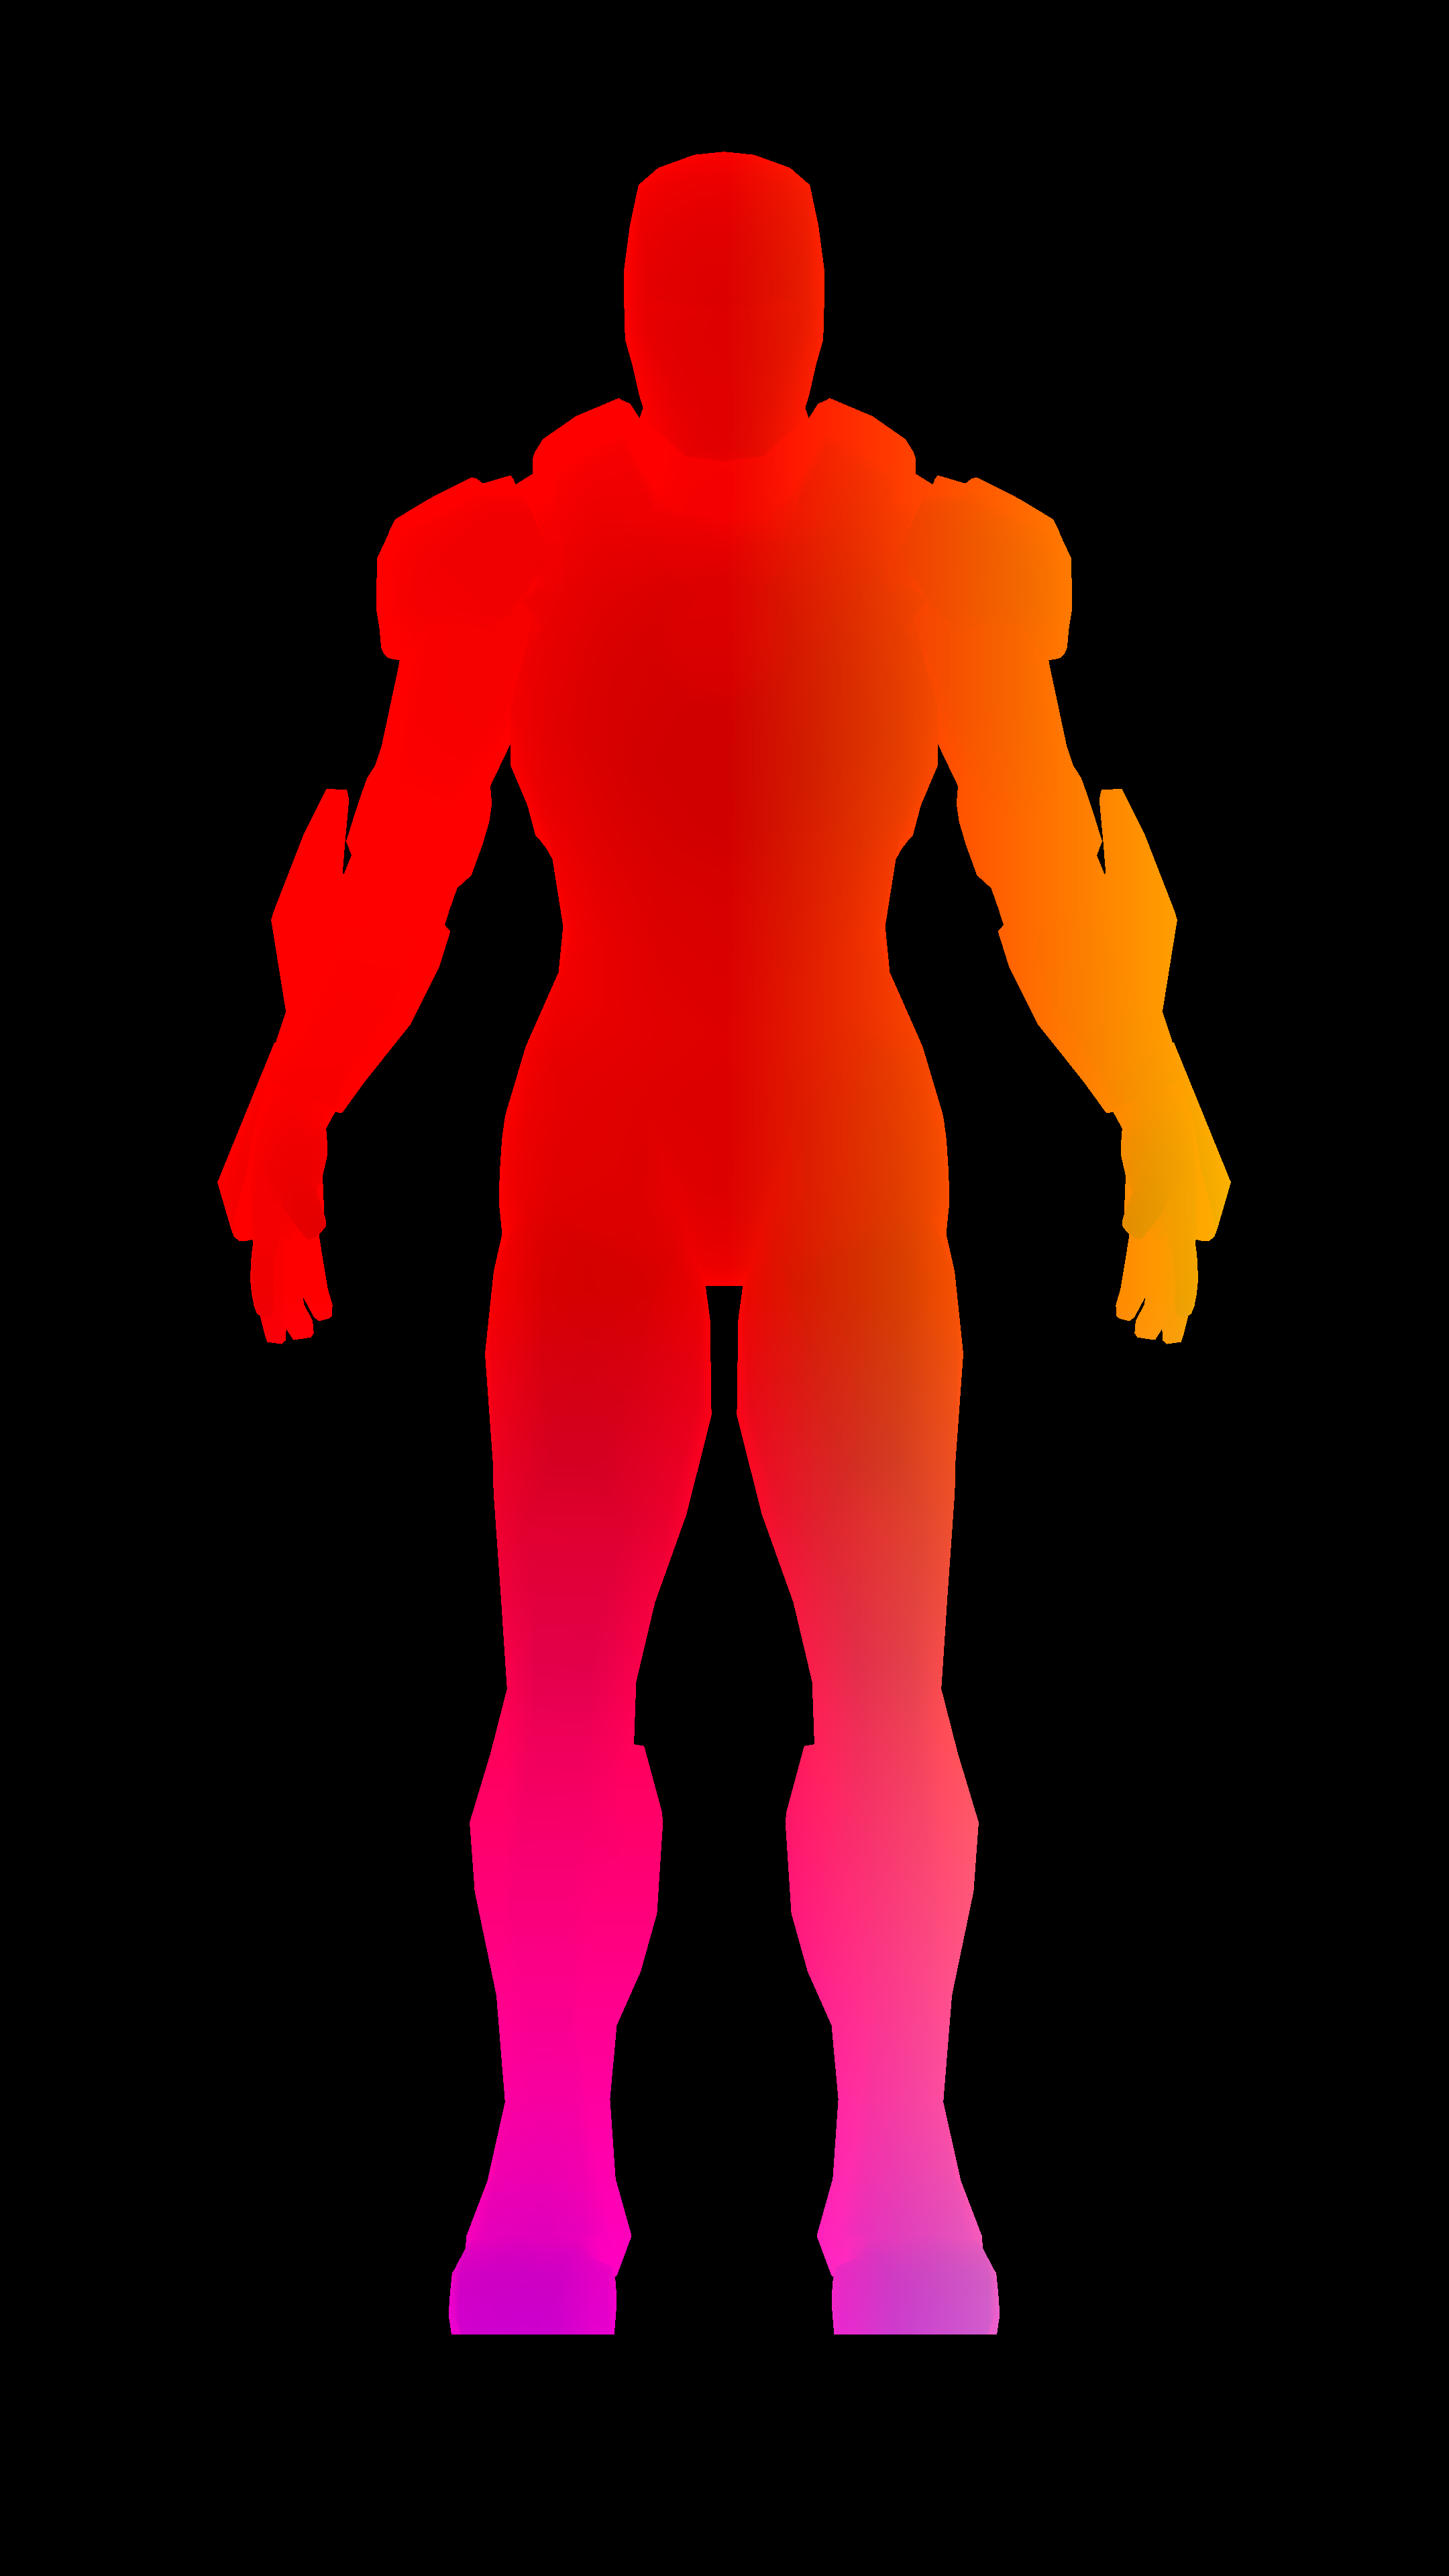
\includegraphics[width=37mm]{img/position}
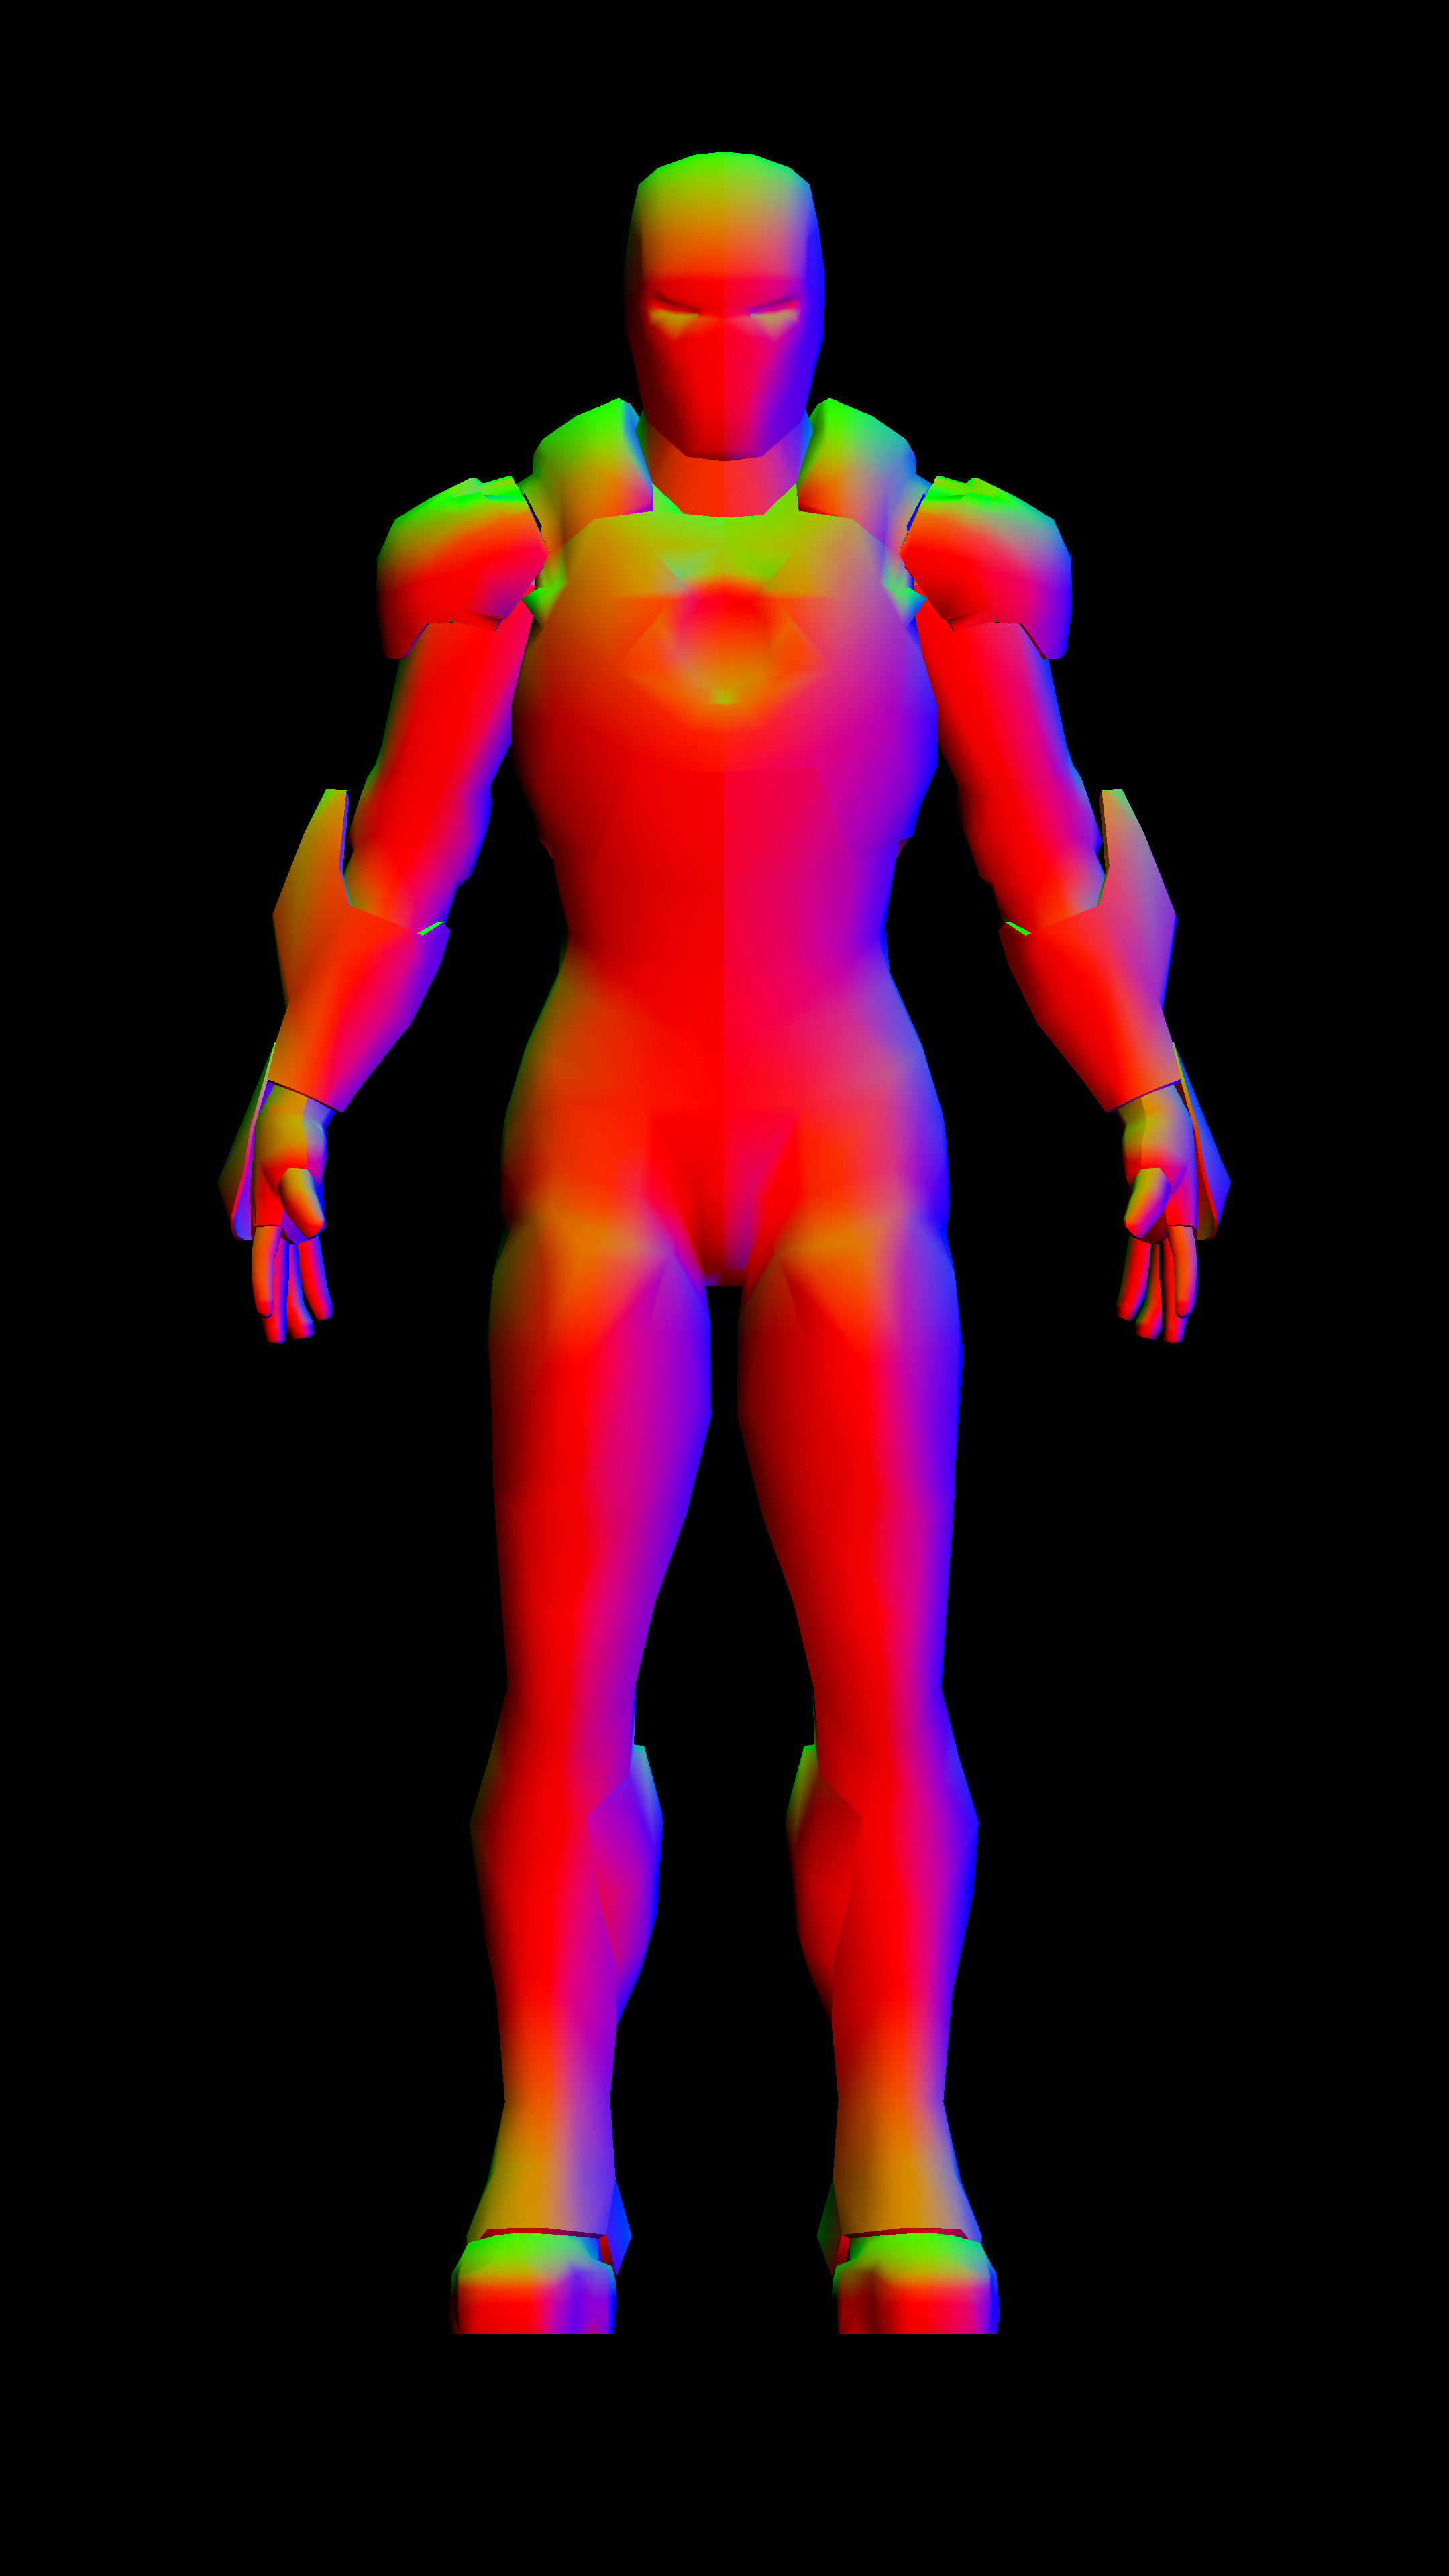
\includegraphics[width=37mm]{img/normal}
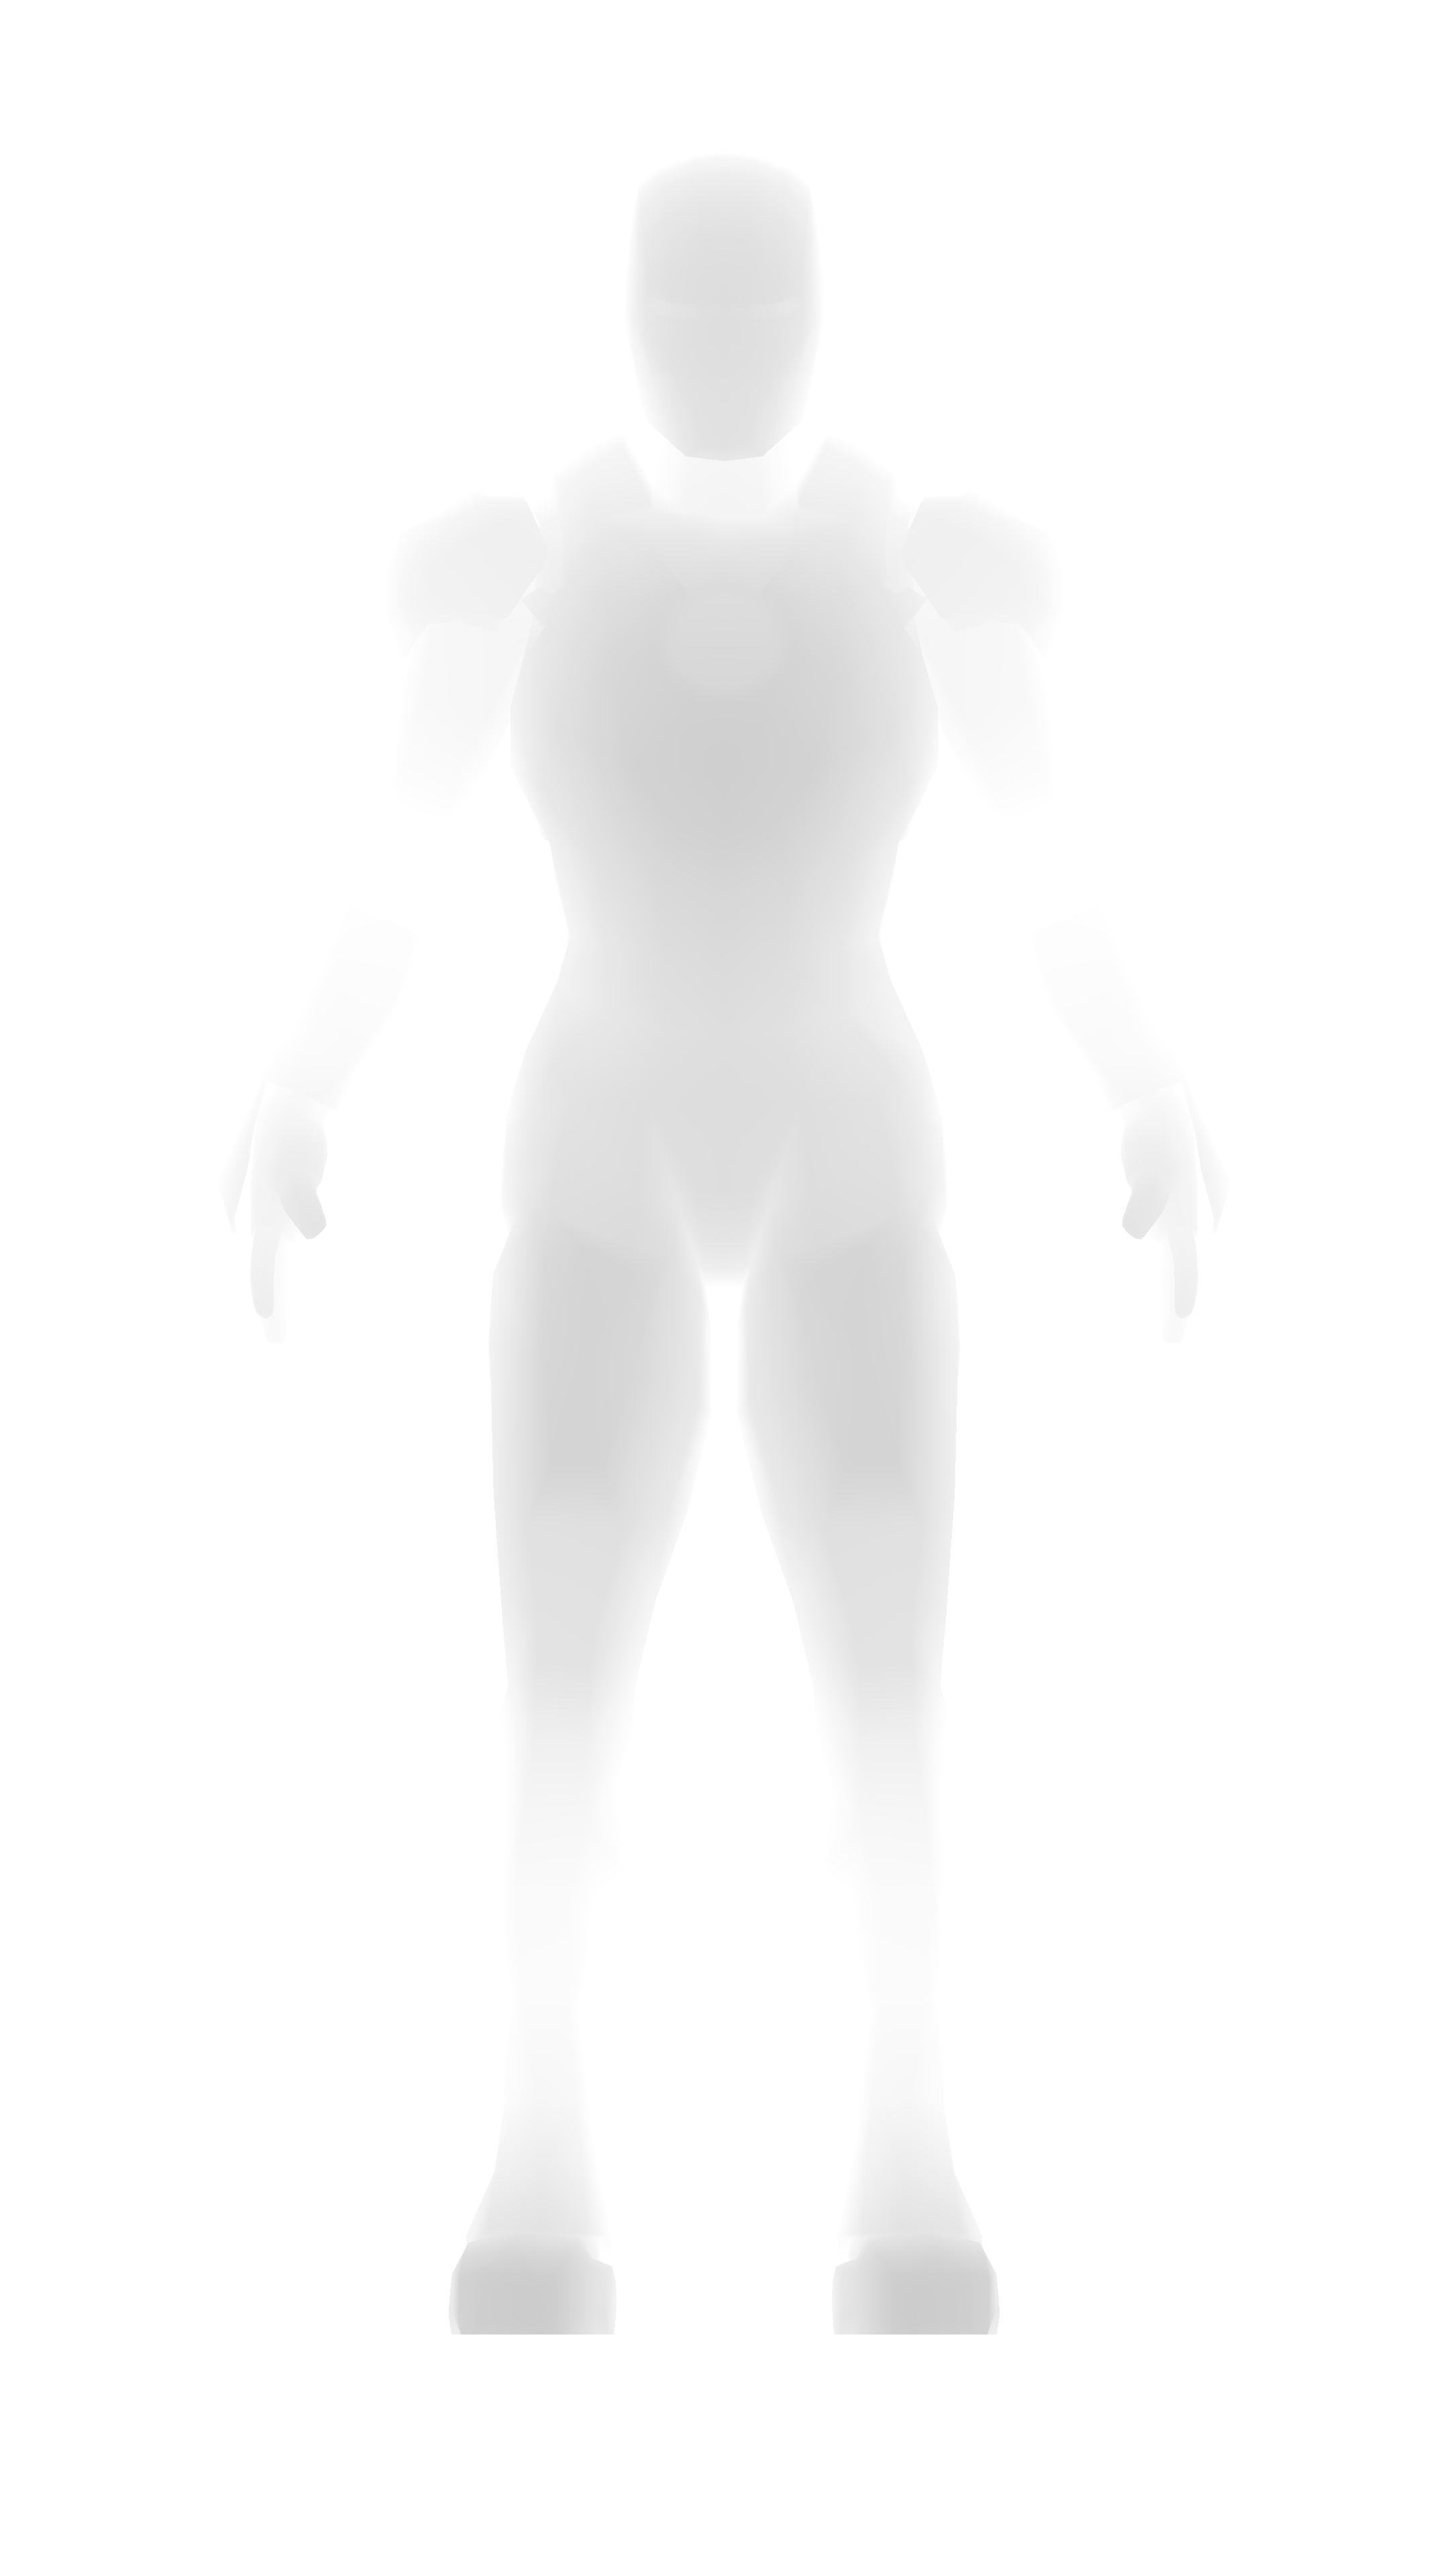
\includegraphics[width=37mm]{img/depth}
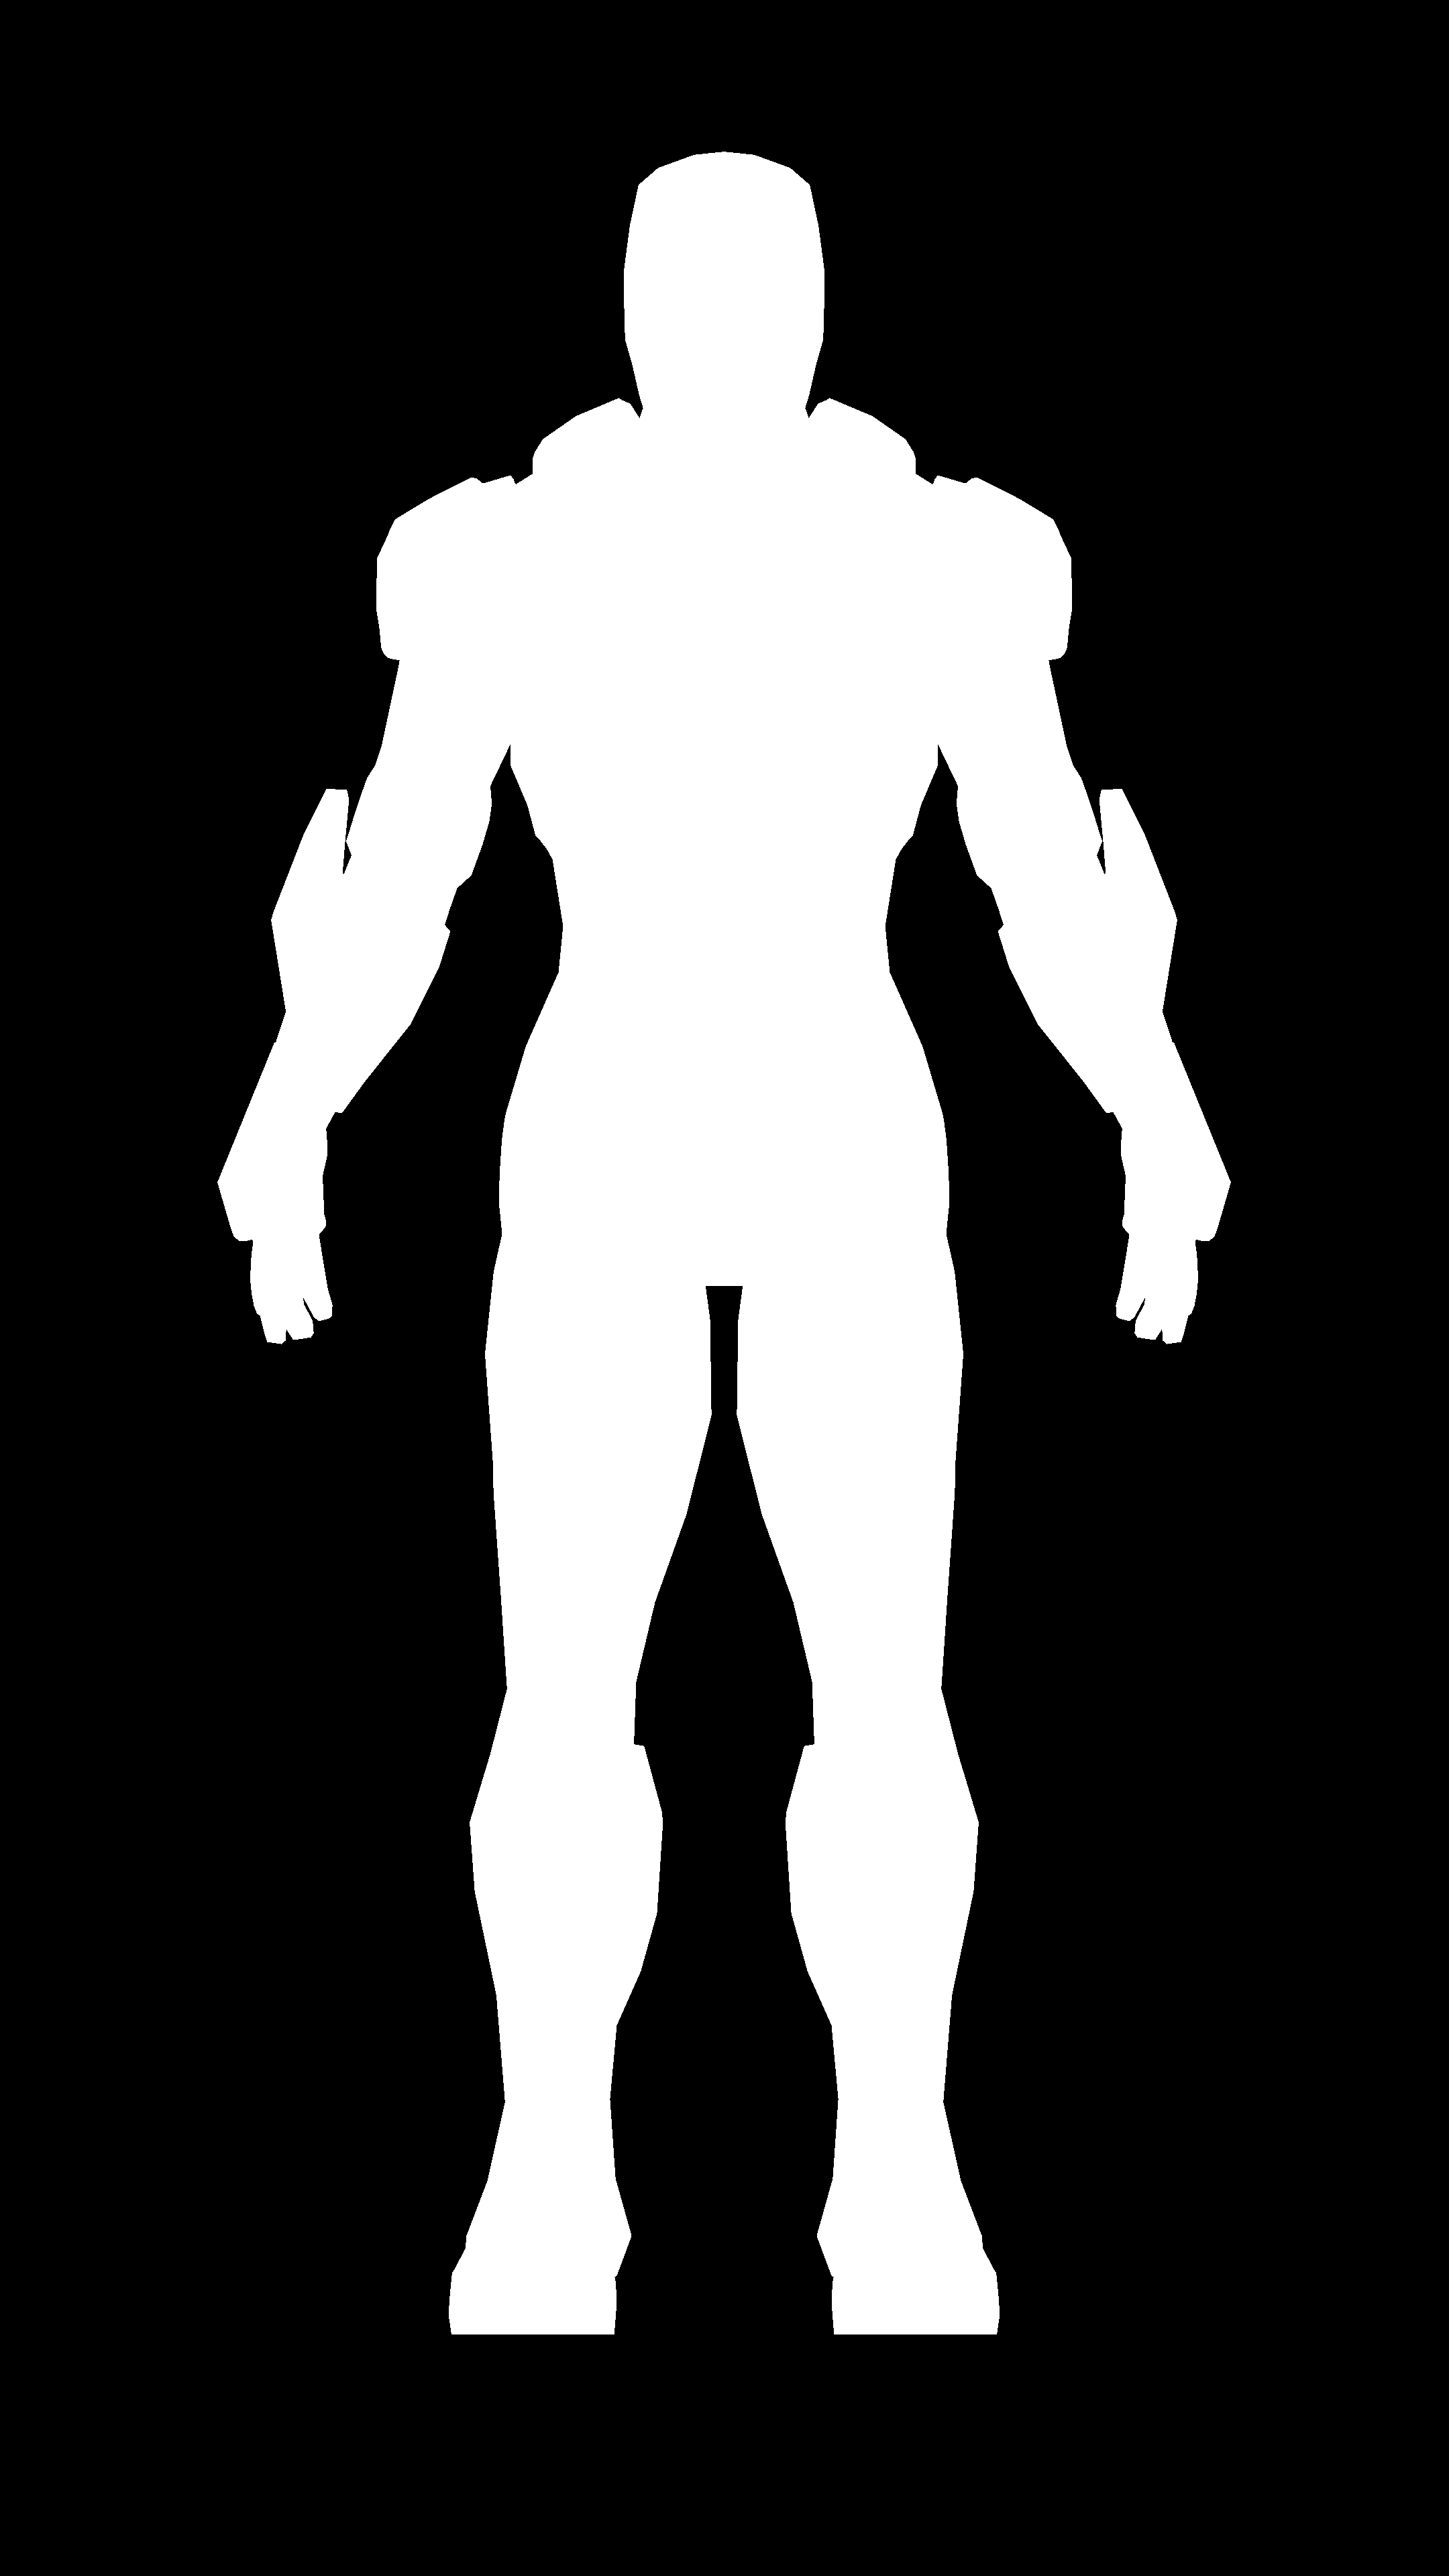
\includegraphics[width=37mm]{img/mask}
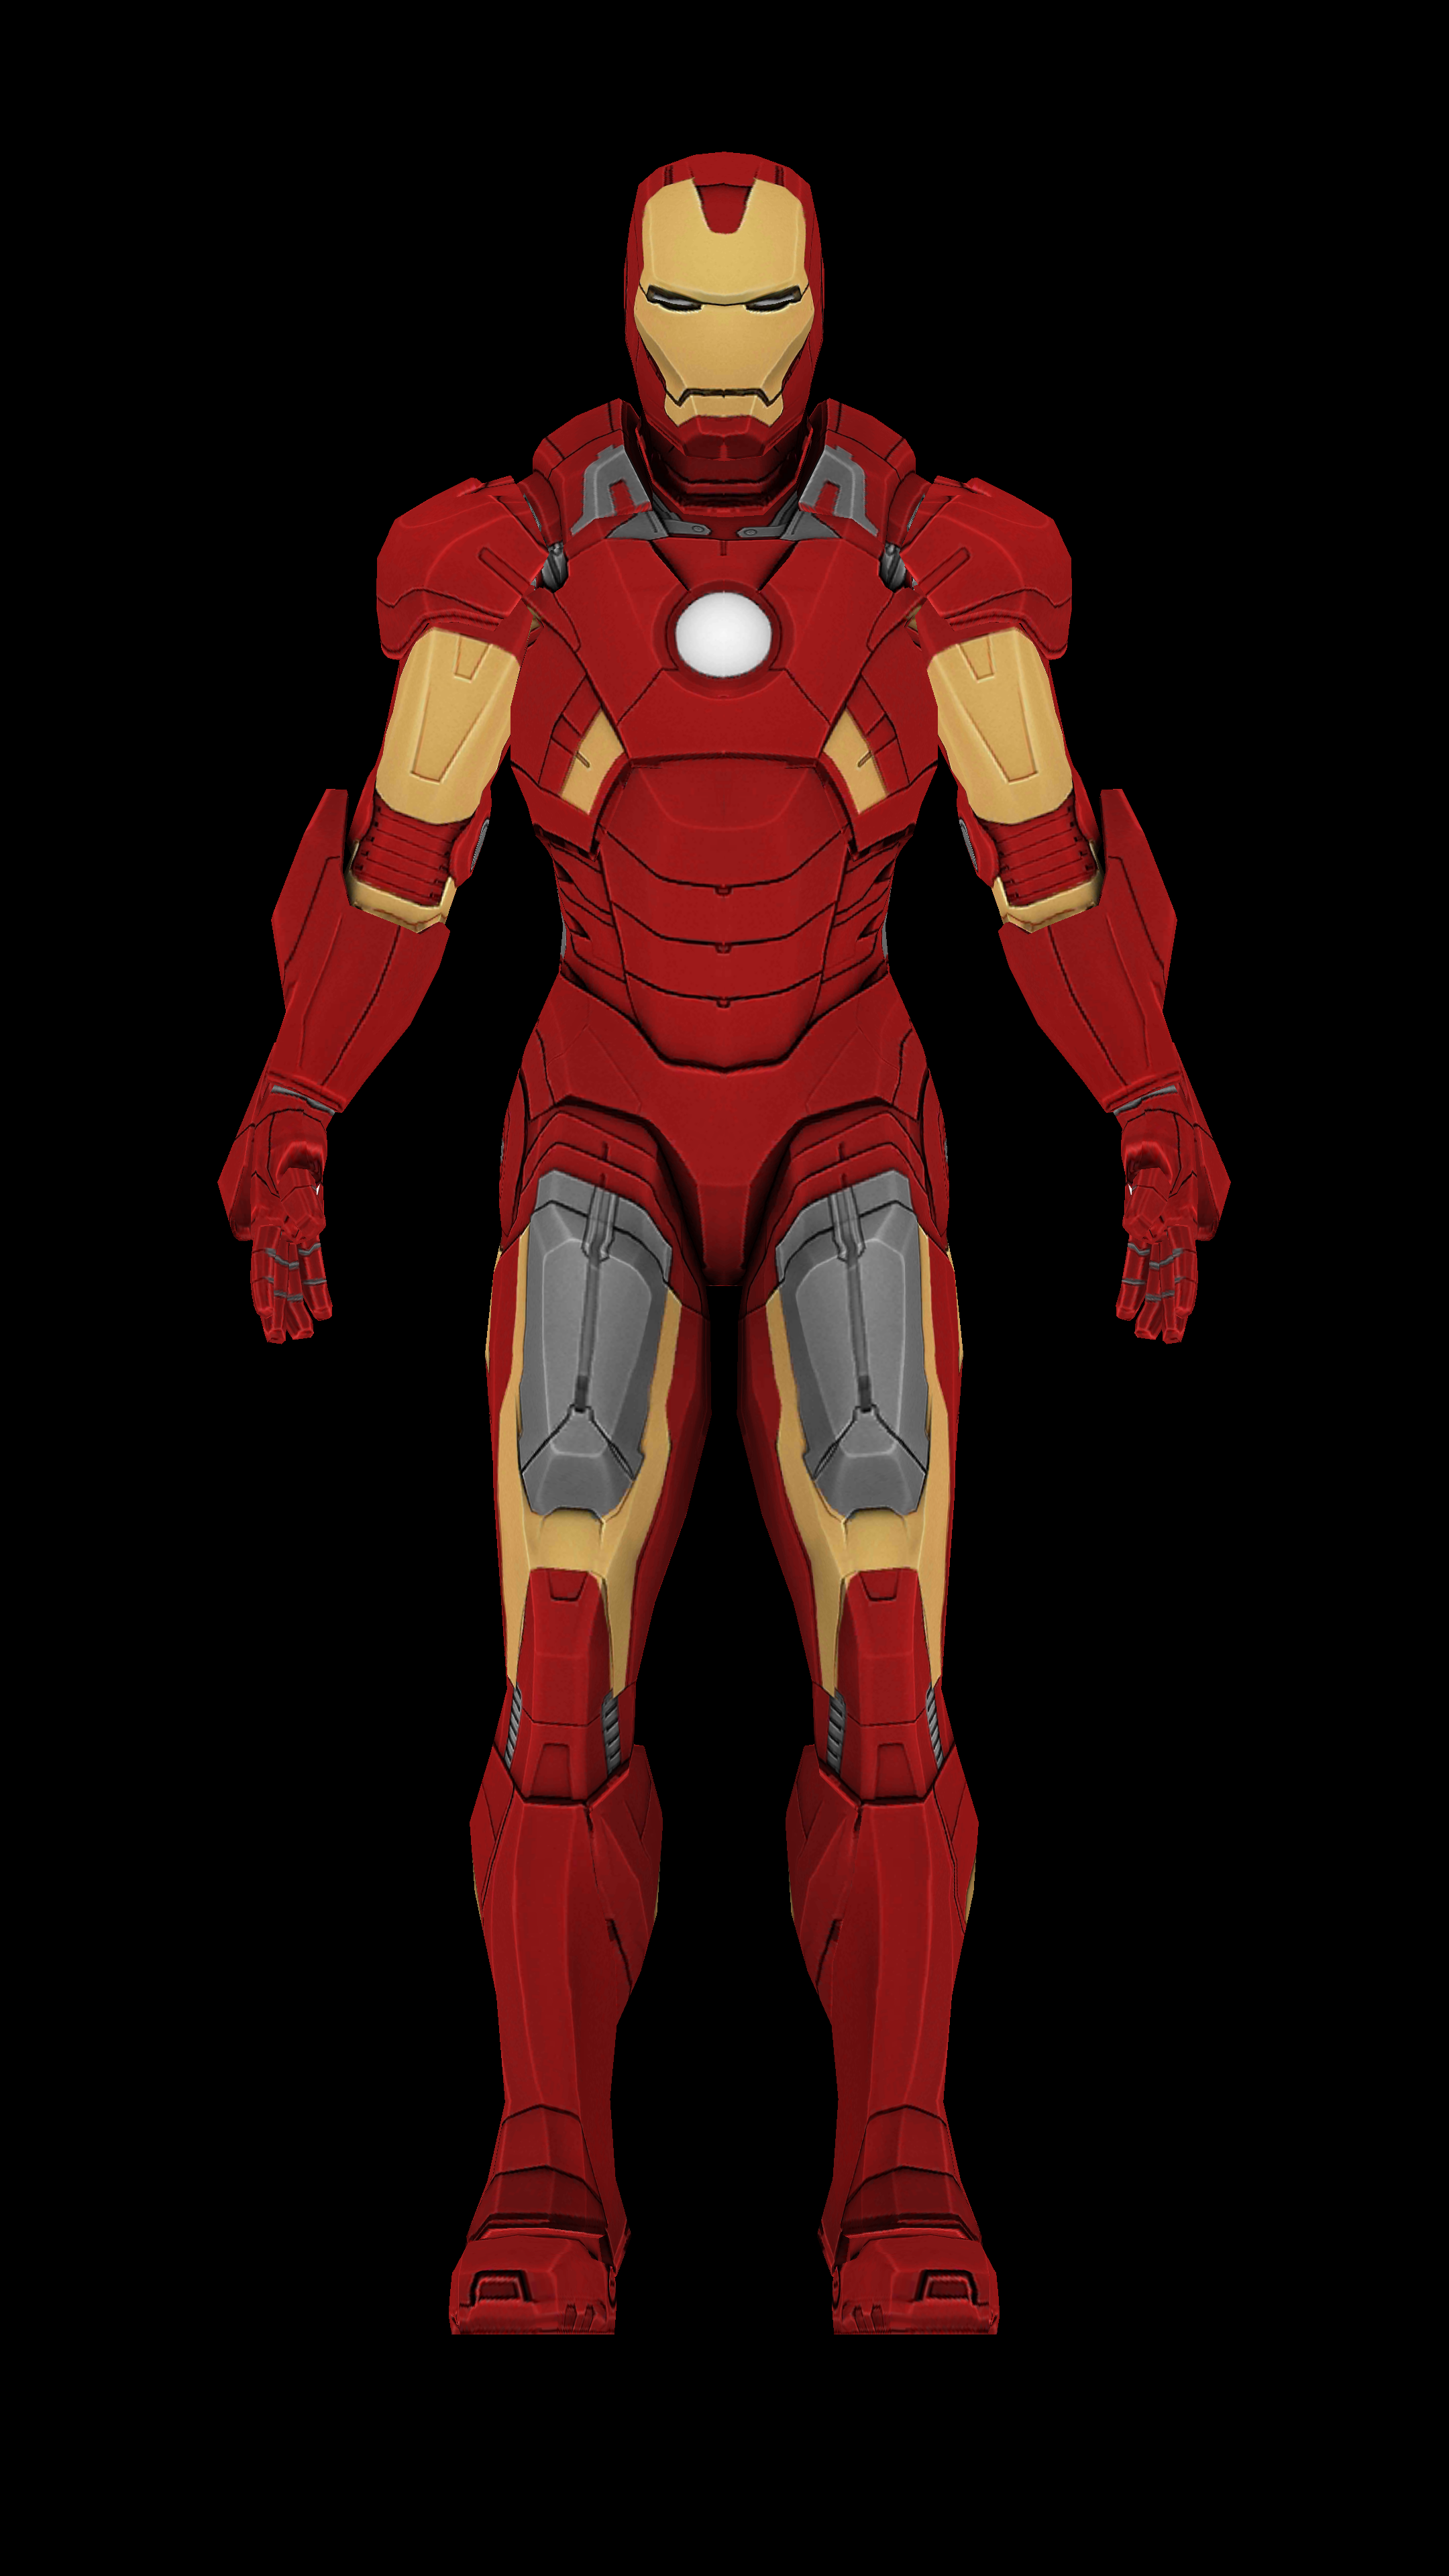
\includegraphics[width=37mm]{img/albedo}
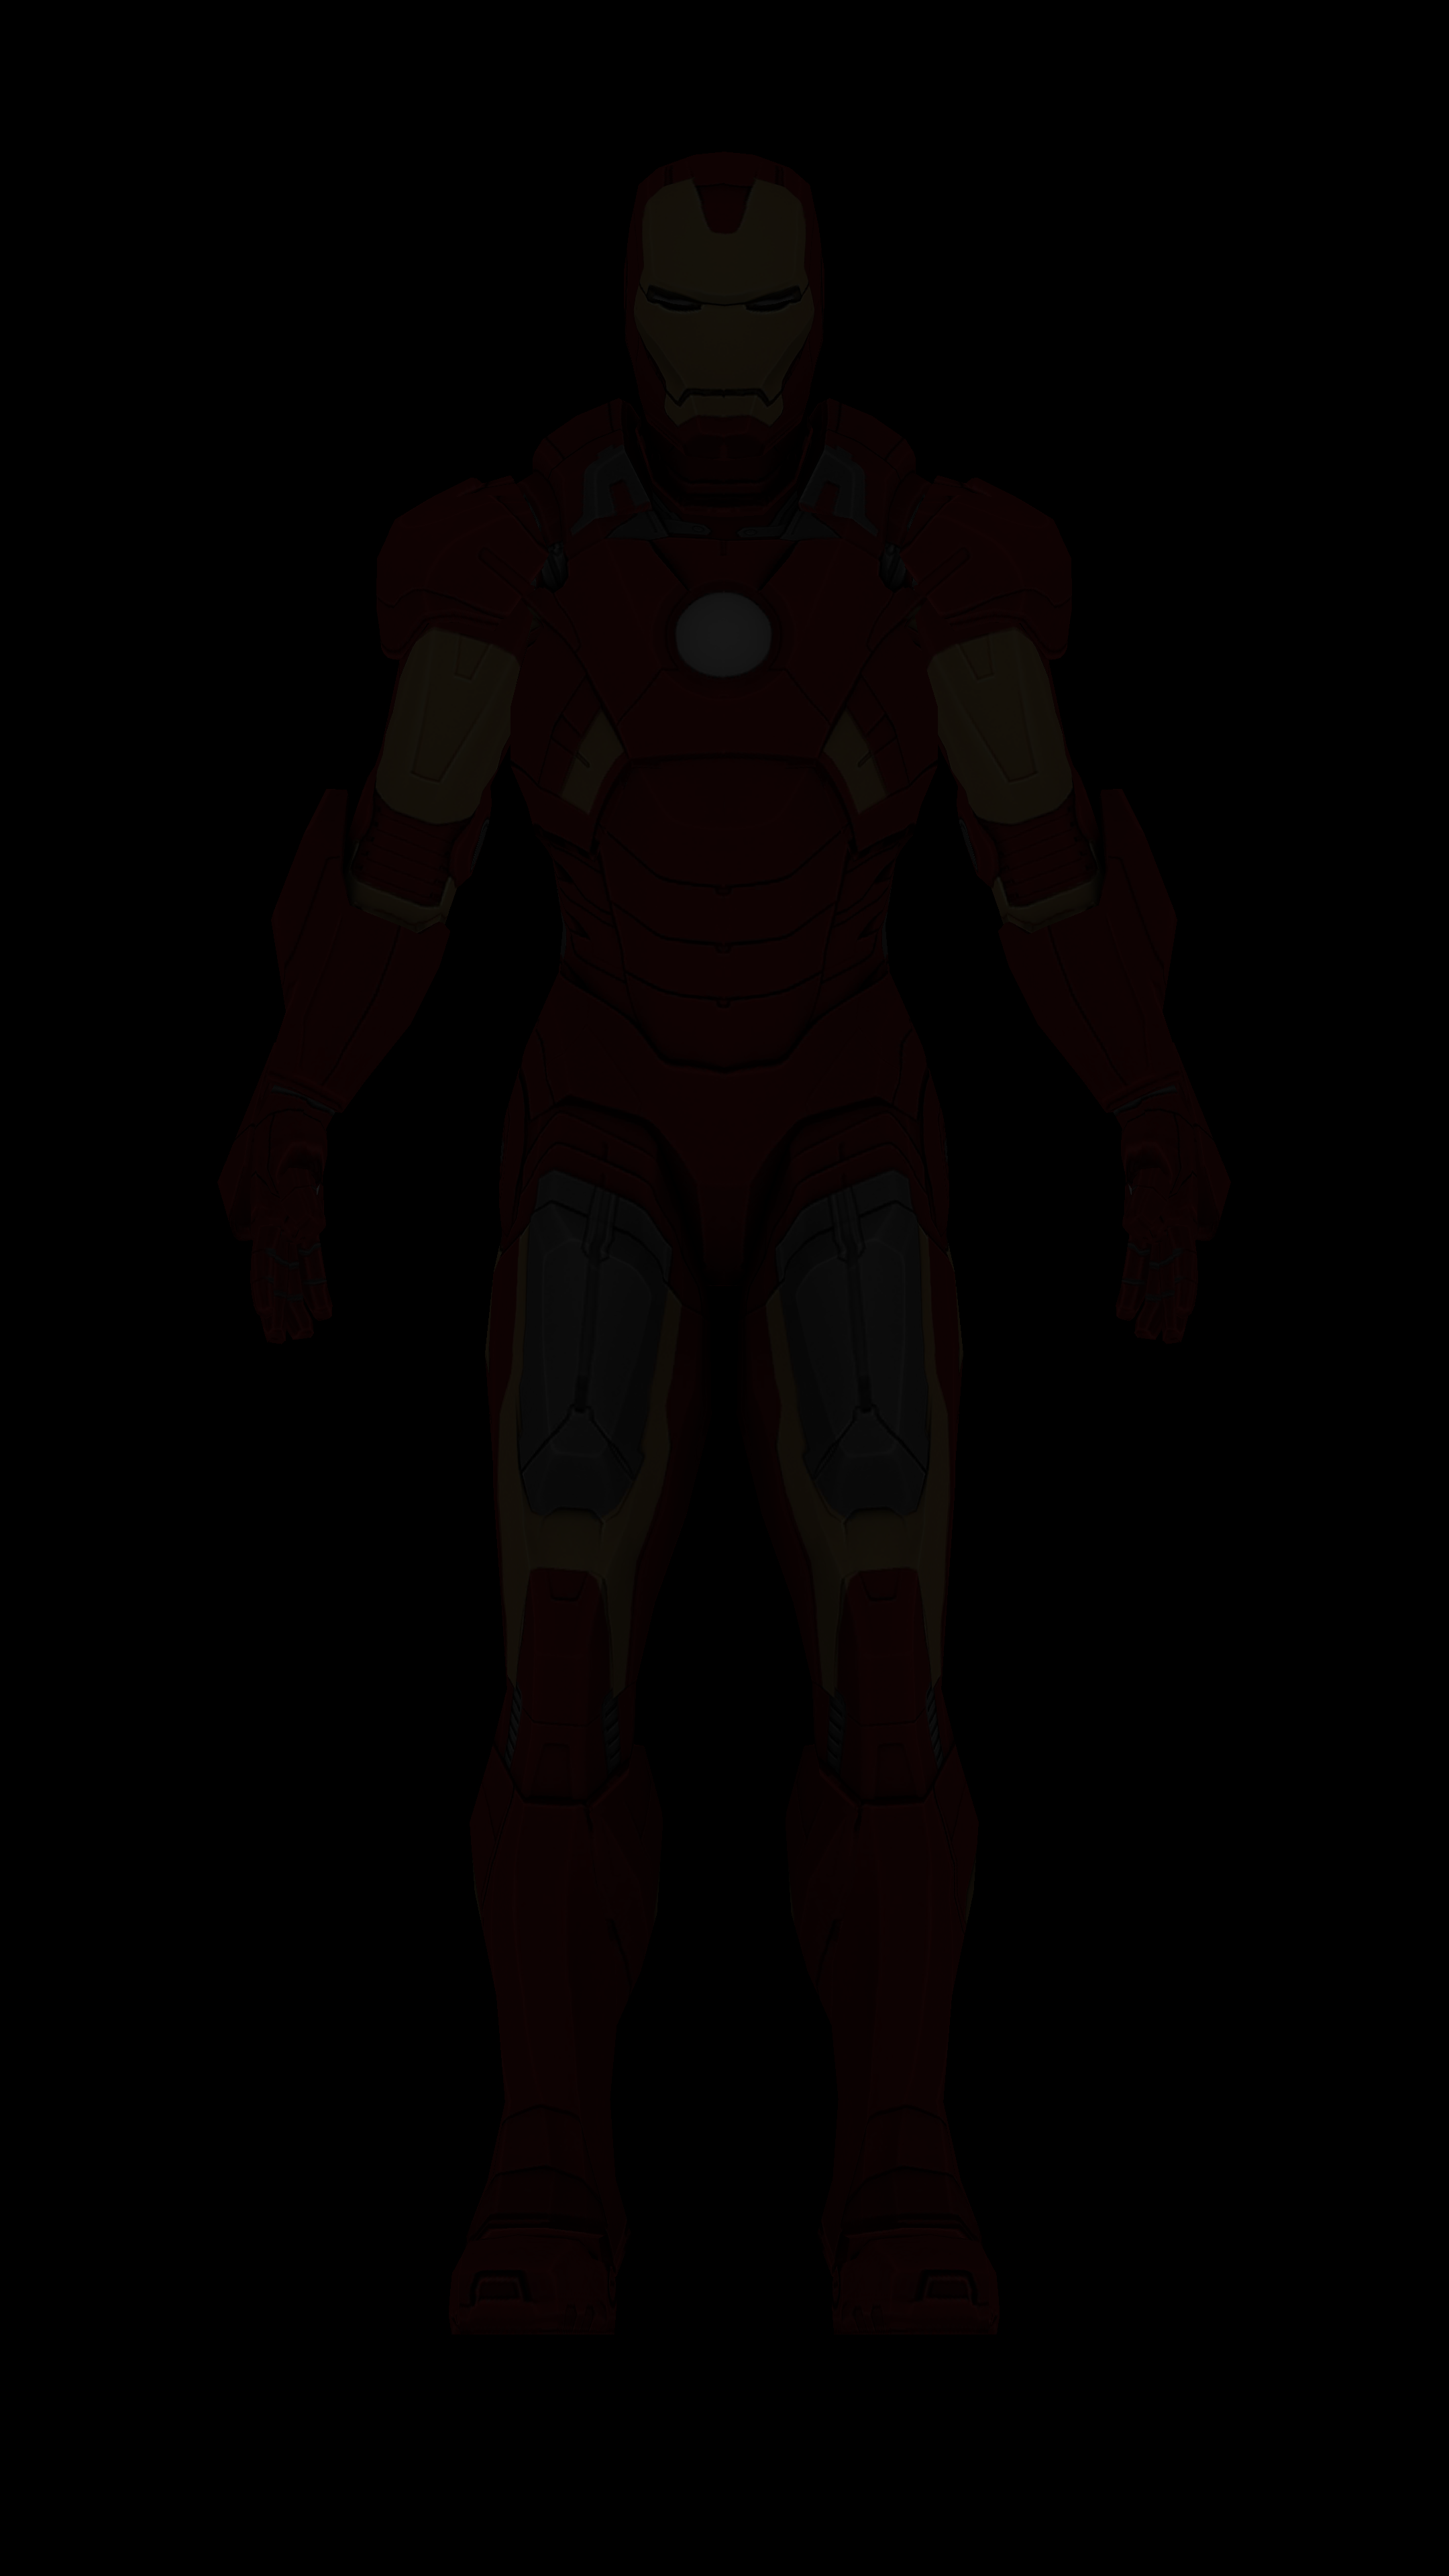
\includegraphics[width=37mm]{img/ambient}
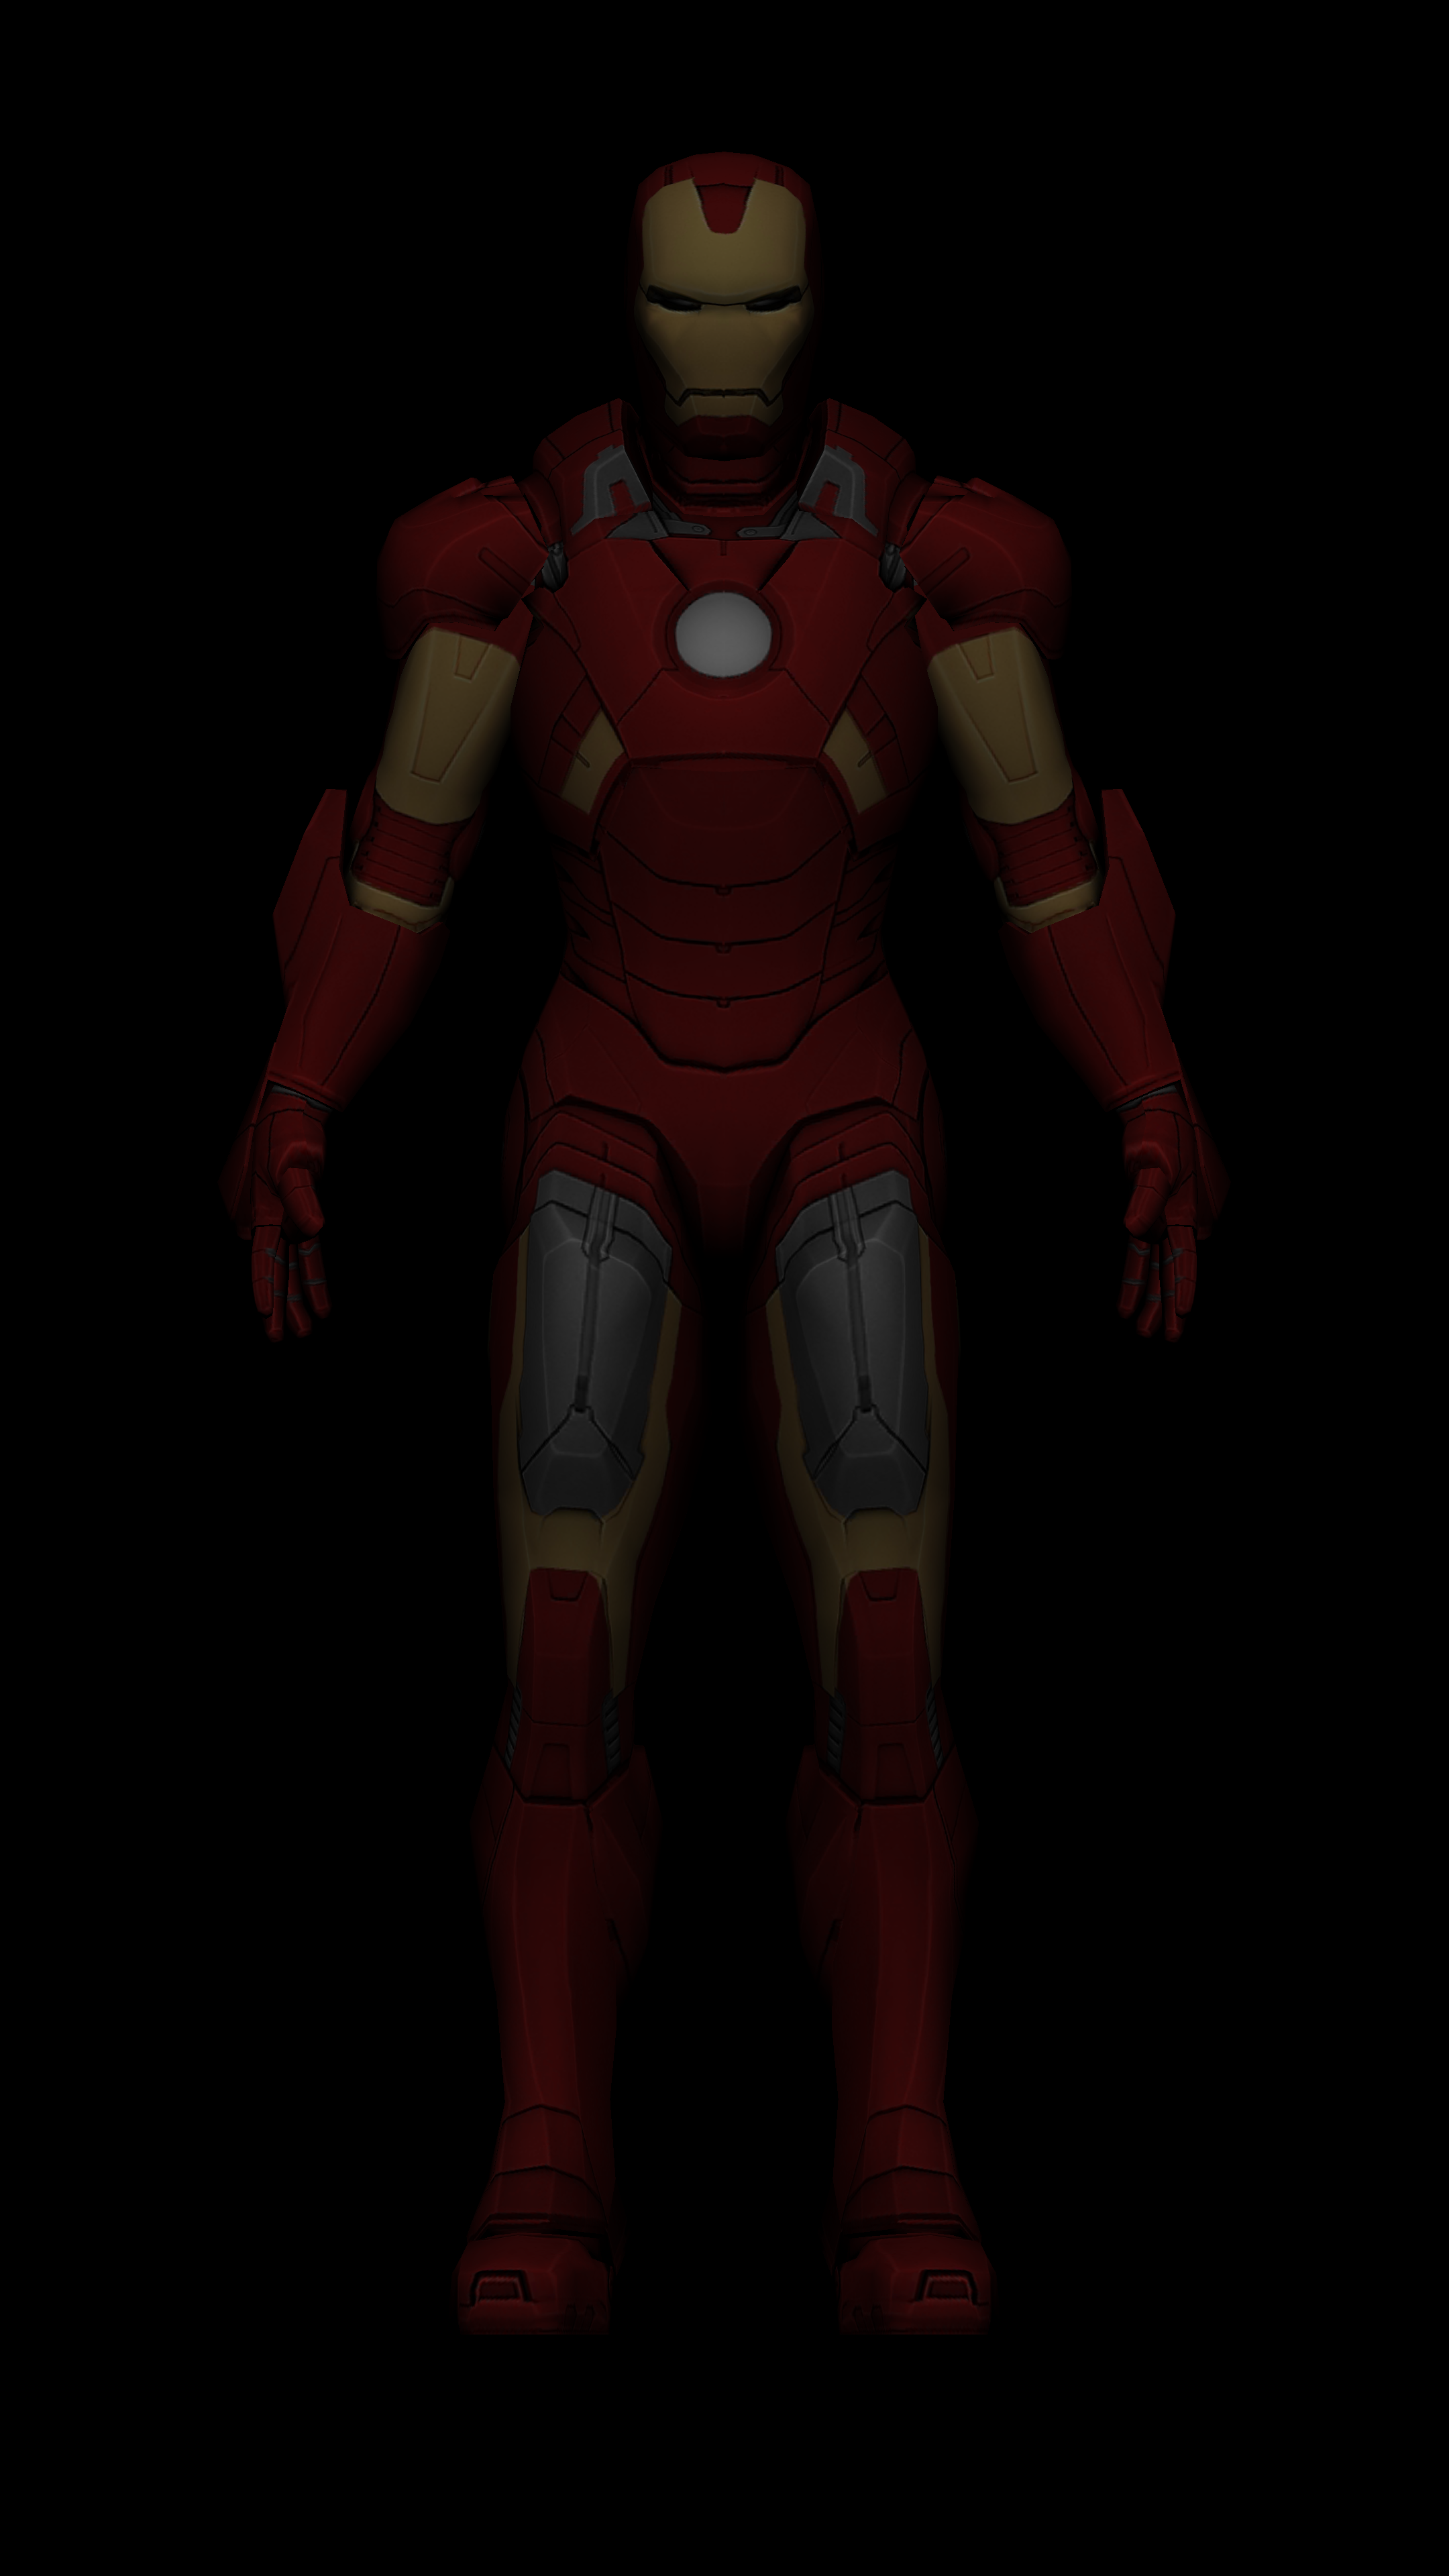
\includegraphics[width=37mm]{img/diffuse}
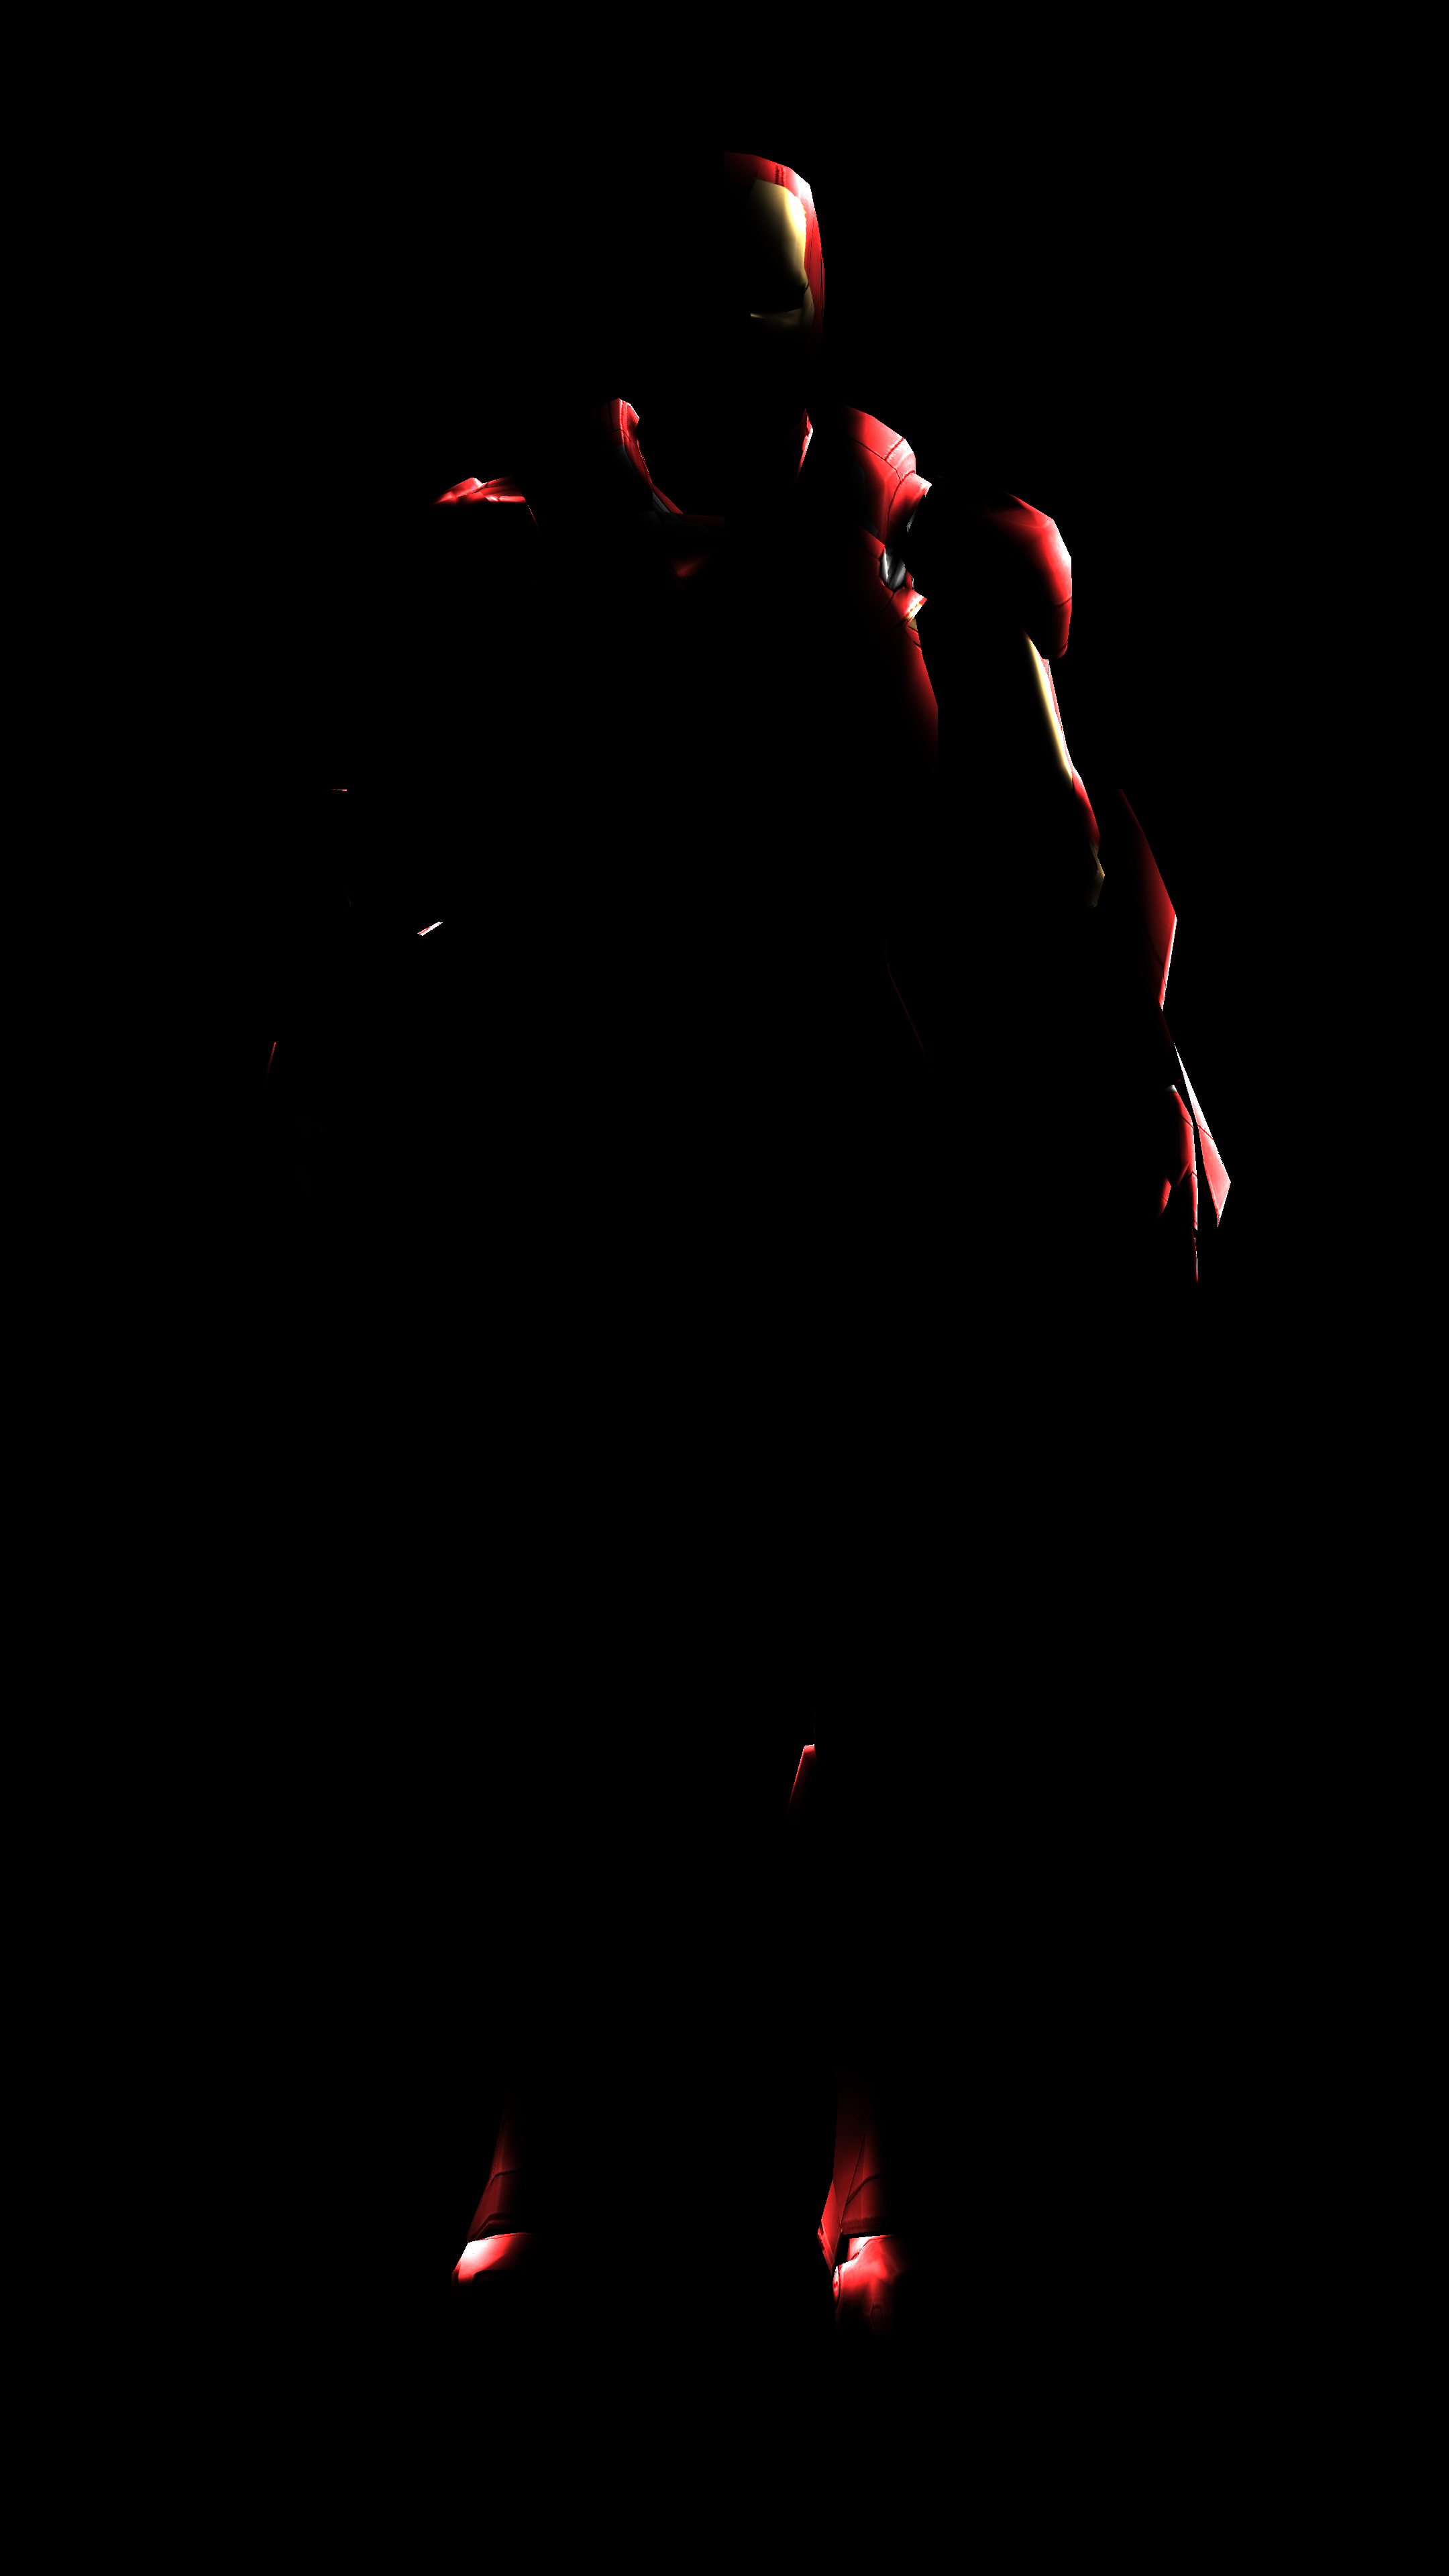
\includegraphics[width=37mm]{img/specular_wet}
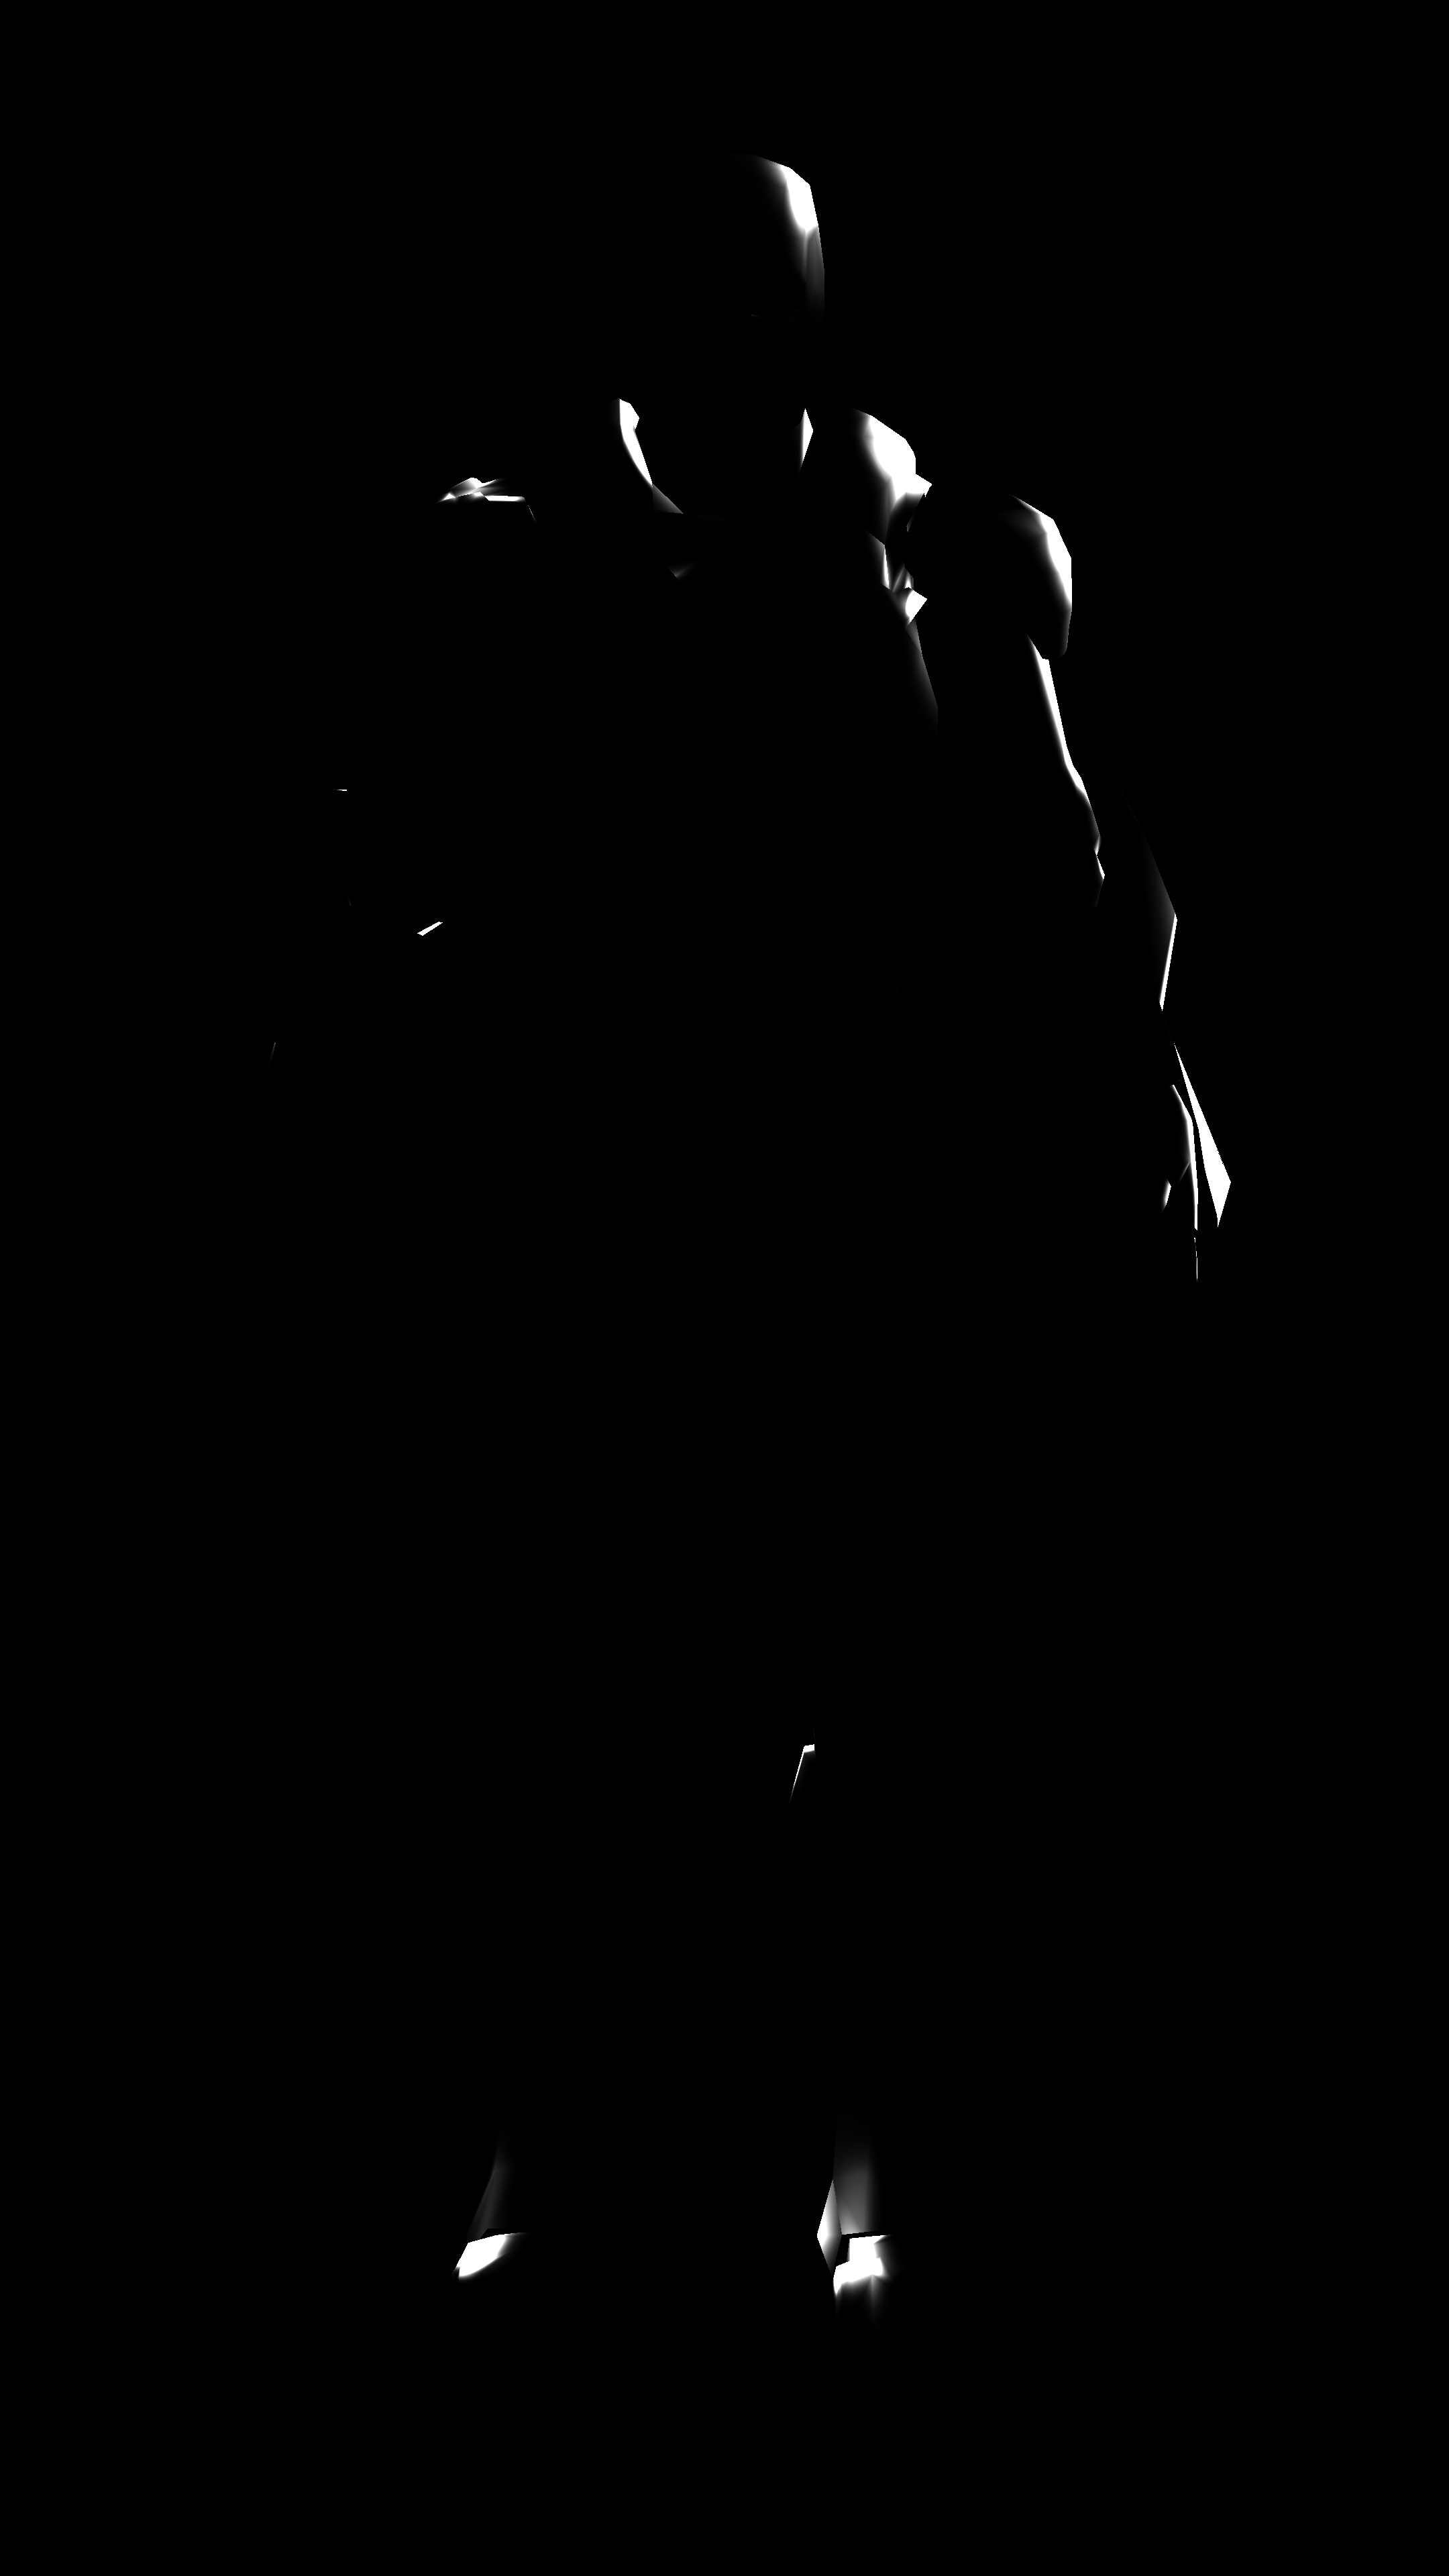
\includegraphics[width=37mm]{img/specular_dry}

\caption{Position, Normal, Depth, Mask, Albedo, Ambient, Diffuse, Specular wet, Specular dry}
\label{mid}
\end{figure}

\section{렌더링 결과}
\begin{figure}[H]
\centering
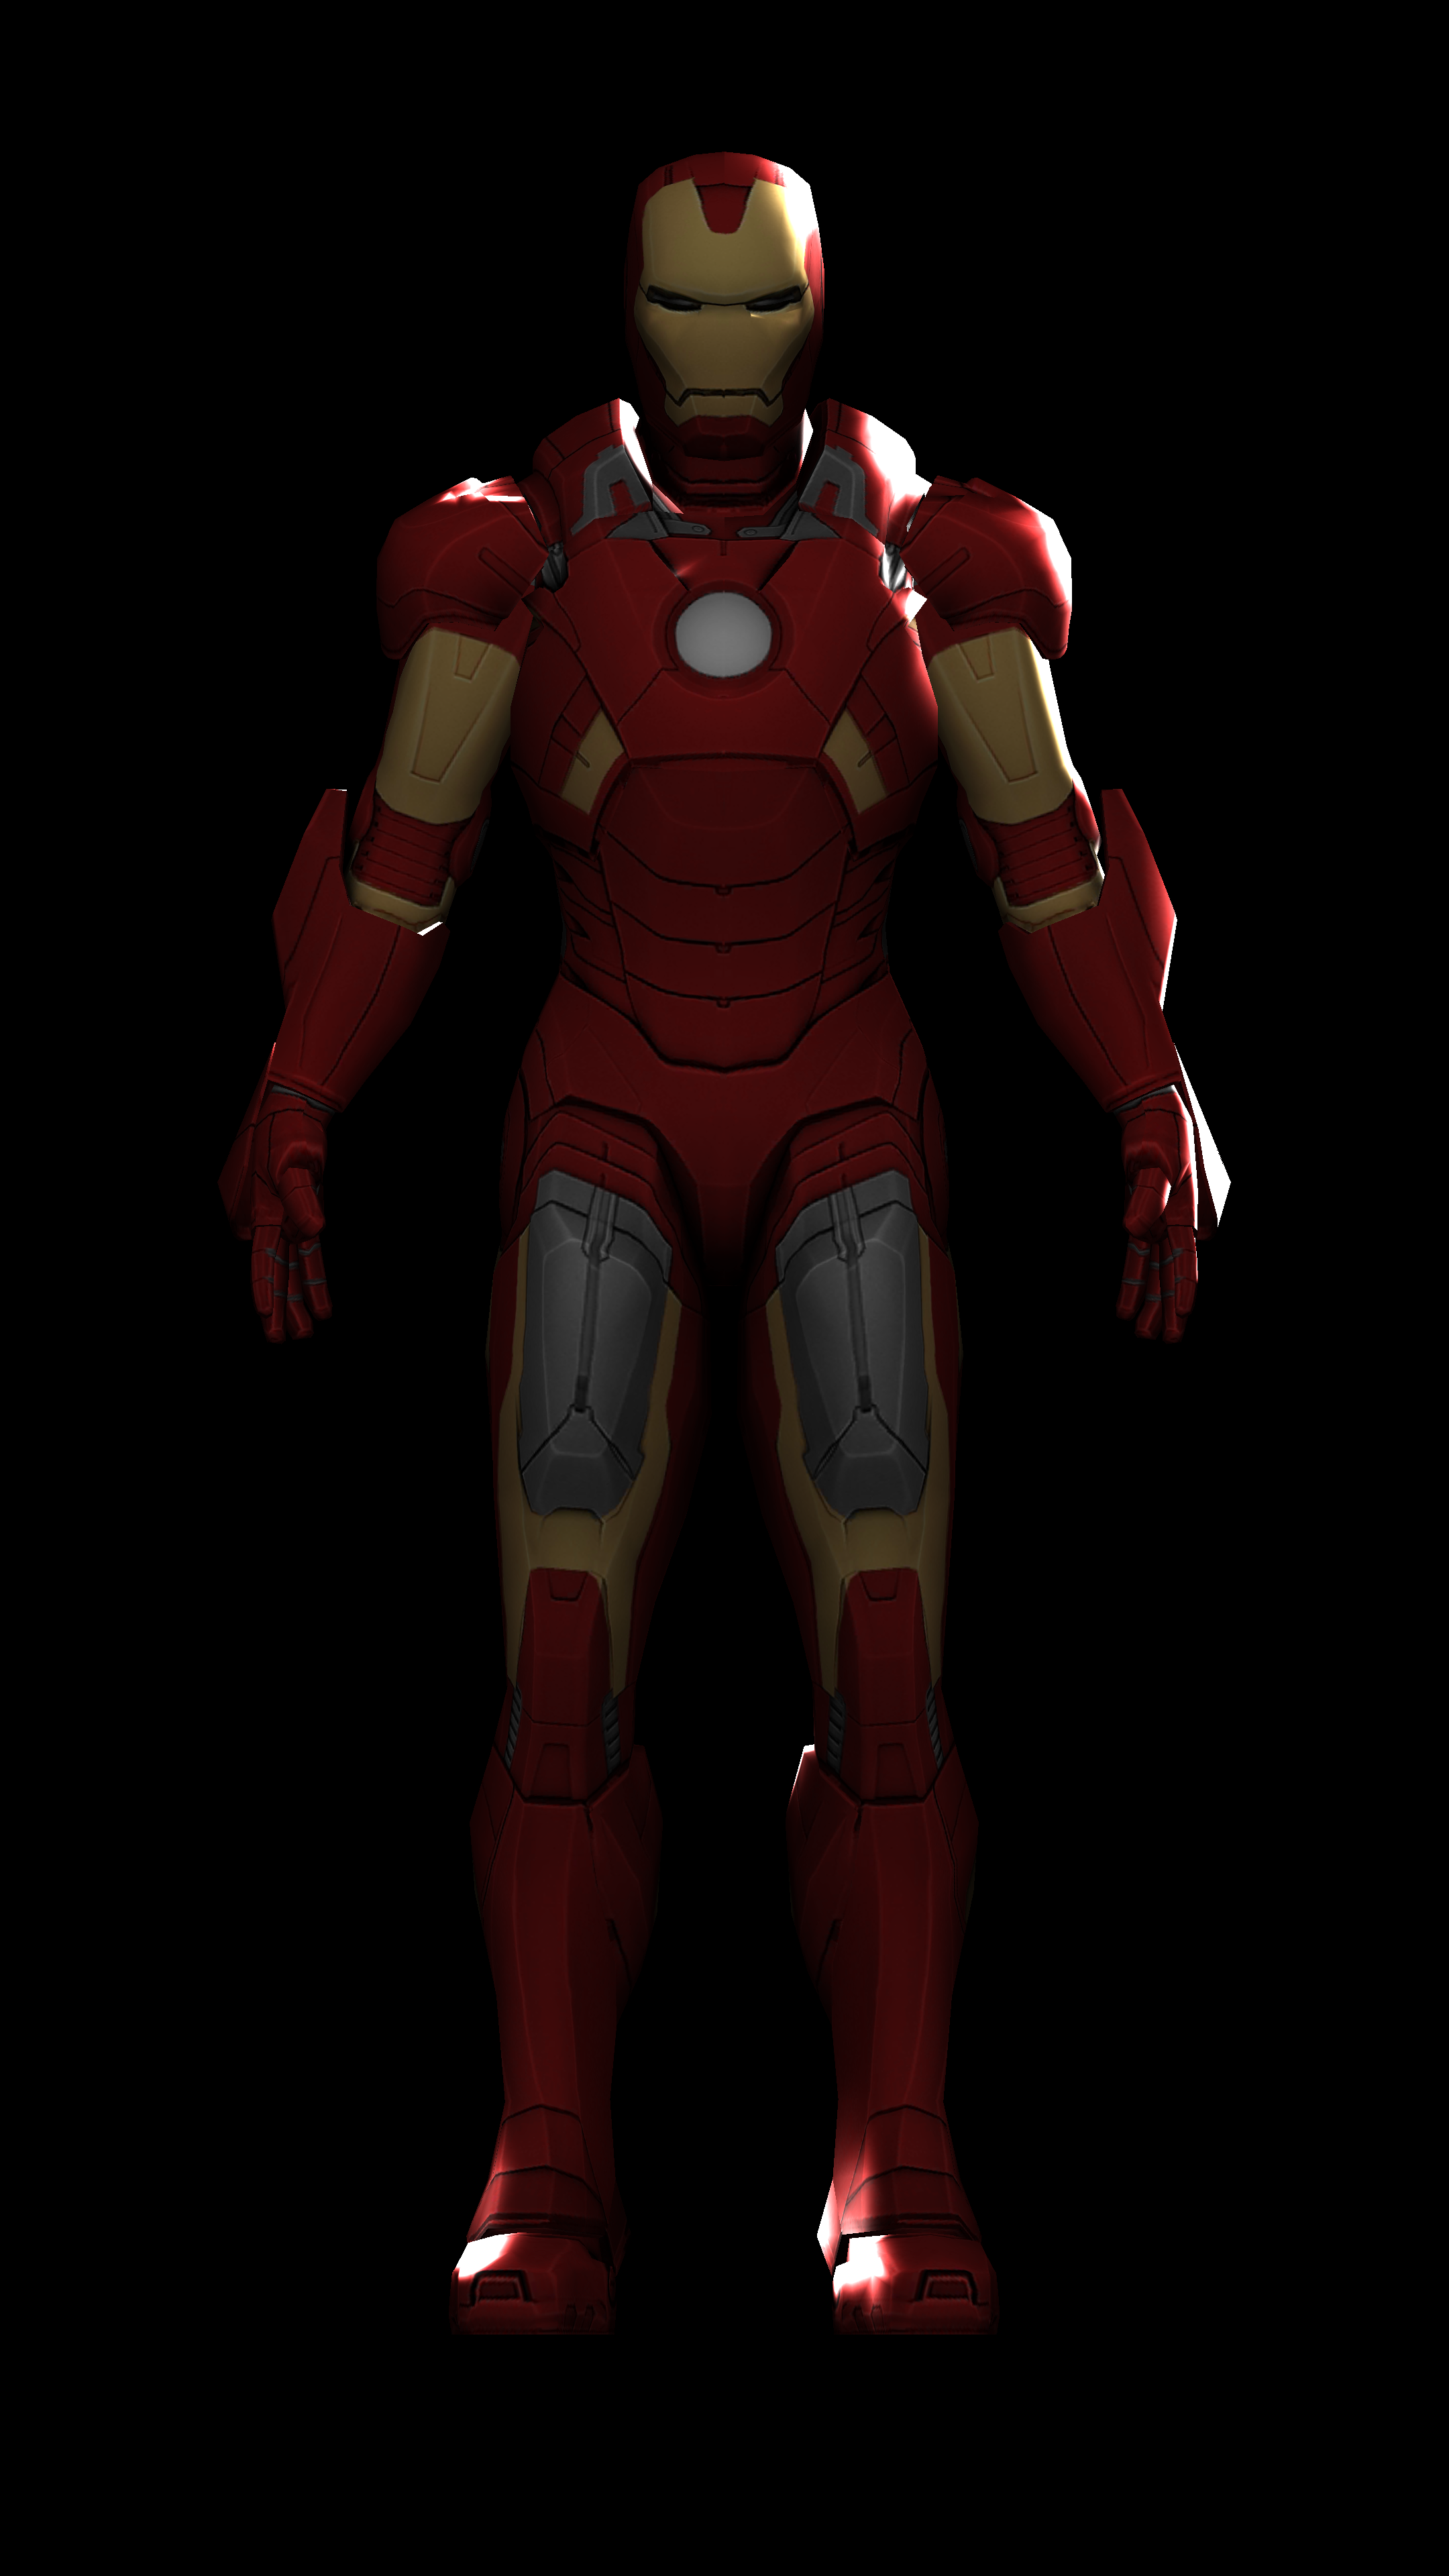
\includegraphics[width=75mm]{img/final}

\caption{Final}
\end{figure}

\section{시스템 성능 측정}

소프트웨어 렌더링은 매우 CPU에 집중적인(CPU-intensive) 응용으로, 시스템 성능을 측정하는 데에 적합하다고 볼 수 있다.
사용 가능한 두 시스템에서 본 프로그램을 수 회 실행하여 수행 시간을 측정하였다.

\begin{figure}
\begin{center}
     \begin{tabular}{| l | l | l | l |}
     \hline
      & i7-2600 데스크톱 & i7-3630QM 노트북 \\ \hline
1&	56249 &	62099 \\ \hline
2&	64657 &	62444 \\ \hline
3&	56049 &	61917 \\ \hline
4&	63277 &	61768 \\ \hline
5&	63722 &	61445 \\ \hline
6&	56177 &	61506 \\ \hline
평균&	60021.83 & 	61863.16 \\ \hline
     \end{tabular}
\caption{두 시스템에서 측정한 렌더링 수행 시간 (단위 : ms)}
\end{center}
\end{figure}


\section{결론}

현대적인 지연 셰이딩 방법이 적용된 소프트웨어 렌더러를 개발하고 테스트하였다. 또, CPU에 의존하는 점을 이용하여
시스템 성능 측정 도구로의 이용 가능성을 살펴보았다. 실제 소스 코드를 작성한 시간은 약 12시간이고
3840 $\times$ 2160 해상도의 24비트 프레임을 렌더링하는 데 걸린 프로그램 수행 시간은 약 60초로,
하드웨어 가속기를 사용하지 않고도 짧은 기간 내에 픽셀 단위 조명이 적용된 만족할 만한 그래픽 품질을 얻을 수 있었다는 것은
호모지니어스 컴퓨팅의 관점에서 대단히 고무적인 일이다.

지연 셰이딩 기법을 사용한 소프트웨어 렌더러는 하드웨어 가속기의 제약 사항을 피할 수 있어
기존 소프트웨어 렌더러 개발 기간과 큰 차이가 없었다. 그래픽 하드웨어를 다루는 기본적인
코드를 작성하지 않아도 되고, 언어를 선택하는 문제에 있어서 소프트웨어 렌더링이 더 자유롭기 때문에,
3D 그래픽과 선형대수를 위해 만들어진 라이브러리를 사용하지 않는 상태에서도 개발 용이성은 더 높게 느껴졌다.
또, 셰이더 코드에 객체 지향과 다형성을 적용할 수 있어 향후 유지 보수에도 유리할 것이다.

앞으로 더 많은 지오메트리와 다양한 조명 모델, 더 복잡한 실시간 응용을 사용하는 제품이 개발되고
시장에 출시될 것이라는 것은 자명하다. 멀지 않은 미래에 한 종류의 프로세서로 실시간 렌더링을 처리하는 프로그램을
작성할 수 있기를 기대해 본다.

\begin{thebibliography}{99}
\bibitem{model} Balmung, Iron Man Mark 7, http://tf3dm.com/3d-model/iron-man-mark-7-81052.html
\bibitem{korea}James D. Foley, Andries van Dam, Steven K. Feiner, John F. Hughes, Richard L. Phillips, 조동섭, 한정현 옮김, 컴퓨터 그래픽스, 홍릉과학출판사, 1998, p.178
\bibitem{rtr} Tomas Akenine-Moller, Eric Haines, Naty Hoffman, Real-Time Rendering, Third Edition, A K Peters, 2008, p.91
\bibitem{kim} 김용준, 3D 게임 프로그래밍, 한빛미디어, 2010, p.182
\bibitem{nvidia} Shawn Hargreaves, Mark Harris, Deferred Shading, NVIDIA, 2004, p.6
\end{thebibliography}

\section*{주제어}
컴퓨터 그래픽스, 3D 렌더링, 소프트웨어 렌더링, 지연 셰이딩, 성능 측정


\end{document}
